\documentclass[floatsintext,doc]{apa6}
\usepackage{lmodern}
\usepackage{amssymb,amsmath}
\usepackage{ifxetex,ifluatex}
\usepackage{apacite}
%\usepackage{hyperref}
\usepackage[utf8]{inputenc}
%\usepackage{fourier}%
%\usepackage{fourier}%
%\usepackage{heuristica}
\usepackage{geometry}

\usepackage{array}
\usepackage{tabularx}
\usepackage{caption}

\usepackage{fixltx2e} % provides \textsubscript
\ifnum 0\ifxetex 1\fi\ifluatex 1\fi=0 % if pdftex
  \usepackage[T1]{fontenc}
  \usepackage[utf8]{inputenc}
\else % if luatex or xelatex
  \ifxetex
    \usepackage{mathspec}
  \else
    \usepackage{fontspec}
  \fi
  \defaultfontfeatures{Ligatures=TeX,Scale=MatchLowercase}
\fi
% use upquote if available, for straight quotes in verbatim environments
\IfFileExists{upquote.sty}{\usepackage{upquote}}{}
% use microtype if available
\IfFileExists{microtype.sty}{%
\usepackage{microtype}
\UseMicrotypeSet[protrusion]{basicmath} % disable protrusion for tt fonts
}{}

%\hypersetup{unicode=true,
%            pdftitle={Not unreasonable: Uncertainty in the language of logic},
%            pdfauthor={Michael Henry Tessler~\& Michael Franke},
%            pdfkeywords={semantics; pragmatics; negation; Bayesian cognitive model; Rational Speech Act},
%            pdfborder={0 0 0},
%            breaklinks=true}
%\urlstyle{same}  % don't use monospace font for urls
\usepackage{graphicx,grffile}
\makeatletter
\def\maxwidth{\ifdim\Gin@nat@width>\linewidth\linewidth\else\Gin@nat@width\fi}
\def\maxheight{\ifdim\Gin@nat@height>\textheight\textheight\else\Gin@nat@height\fi}
\makeatother
% Scale images if necessary, so that they will not overflow the page
% margins by default, and it is still possible to overwrite the defaults
% using explicit options in \includegraphics[width, height, ...]{}
\setkeys{Gin}{width=\maxwidth,height=\maxheight,keepaspectratio}
\IfFileExists{parskip.sty}{%
\usepackage{parskip}
}{% else
\setlength{\parindent}{0pt}
\setlength{\parskip}{6pt plus 2pt minus 1pt}
}
\setlength{\emergencystretch}{3em}  % prevent overfull lines
\providecommand{\tightlist}{%
  \setlength{\itemsep}{0pt}\setlength{\parskip}{0pt}}
\setcounter{secnumdepth}{0}
% Redefines (sub)paragraphs to behave more like sections
\ifx\paragraph\undefined\else
\let\oldparagraph\paragraph
\renewcommand{\paragraph}[1]{\oldparagraph{#1}\mbox{}}
\fi
\ifx\subparagraph\undefined\else
\let\oldsubparagraph\subparagraph
\renewcommand{\subparagraph}[1]{\oldsubparagraph{#1}\mbox{}}
\fi

%%% Use protect on footnotes to avoid problems with footnotes in titles
\let\rmarkdownfootnote\footnote%
\def\footnote{\protect\rmarkdownfootnote}



% these packages are needed to insert results 
% obtained from R into the LaTeX document
\usepackage{pgfplotstable}
\usepackage{csvsimple}
\usepackage{siunitx}

% set the name of the folder in which the CSV files with 
% information from R is stored
\newcommand{\datafoldername}{csv_data_4_tex}

% the following code defines the convenience functions
% as described in the main text below

% rlgetvalue returns whatever is the in cell of the CSV file
% be it string or number; it does not format anything
\newcommand{\rlgetvalue}[4]{\csvreader[filter strcmp={\mykey}{#3},
             late after line = {{,}\ }, late after last line = {{}}]
            {\datafoldername/#1}{#2=\mykey,#4=\myvalue}{\myvalue}}

% rlgetvariable is a shortcut for a specific CSV file (myvars.csv) in which
% individual variables that do not belong to a larger chunk can be stored
\newcommand{\rlgetvariable}[1]{\csvreader[]{\datafoldername/myvars.csv}{#1=\myvar}{\myvar}\xspace}

% rlnum format a decimal number
\newcommand{\rlnum}[2]{\num[output-decimal-marker={.},
                             exponent-product = \cdot,
                             round-mode=places,
                             round-precision=#2,
                             group-digits=false]{#1}}

\newcommand{\rlnumsci}[2]{\num[output-decimal-marker={.},
                          scientific-notation = true,
                             exponent-product = \cdot,
                             round-mode=places,
                             round-precision=#2,
                             group-digits=false]{#1}}

\newcommand{\rlgetnum}[5]{\csvreader[filter strcmp={\mykey}{#3},
             late after line = {{,}\ }, late after last line = {{}}]
            {\datafoldername/#1}{#2=\mykey,#4=\myvalue}{\rlnum{\myvalue}{#5}}}

\newcommand{\rlgetnumsci}[5]{\csvreader[filter strcmp={\mykey}{#3},
             late after line = {{,}\ }, late after last line = {{}}]
            {\datafoldername/#1}{#2=\mykey,#4=\myvalue}{\rlnumsci{\myvalue}{#5}}}

\renewcommand{\thetable}{S\arabic{table}}   
\renewcommand{\thefigure}{S\arabic{figure}}

%  \title{Not unreasonable: Uncertainty in the language of negation}
%  \title{Not unreasonable: Multiple opposite meanings are entertained when understanding negation}
%\title{Not stating the opposite: Double negations result in nonredundant meanings}
\title{Supplementary Information\\Not unreasonable: Why two negatives don't make a positive}
    \author{Michael Henry Tessler\textsuperscript{1, 3}~\& Michael Franke\textsuperscript{2}}
    \date{}
  
\shorttitle{SOM-R: Uncertain logical language}
\affiliation{
\vspace{0.5cm}

\textsuperscript{1} Massachusetts Institute of Technology, Department of Brain and Cognitive Sciences\\\textsuperscript{2} University of Osnabr\"{u}ck, Department of Cognitive Science\\\textsuperscript{3} Stanford University, Department of Psychology}

\keywords{}
\usepackage{csquotes}
\usepackage{upgreek}
\captionsetup{font=singlespacing,justification=justified}

\usepackage{longtable}
\usepackage{lscape}
\usepackage{multirow}
\usepackage{tabularx}
\usepackage[flushleft]{threeparttable}
\usepackage{threeparttablex}

%\newenvironment{lltable}{\begin{landscape}\begin{center}\begin{ThreePartTable}}{\end{ThreePartTable}\end{center}\end{landscape}}

\makeatletter
\newcommand\LastLTentrywidth{1em}
\newlength\longtablewidth
\setlength{\longtablewidth}{1in}
\newcommand{\getlongtablewidth}{\begingroup \ifcsname LT@\roman{LT@tables}\endcsname \global\longtablewidth=0pt \renewcommand{\LT@entry}[2]{\global\advance\longtablewidth by ##2\relax\gdef\LastLTentrywidth{##2}}\@nameuse{LT@\roman{LT@tables}} \fi \endgroup}


%\DeclareDelayedFloatFlavor{ThreePartTable}{table}
%\DeclareDelayedFloatFlavor{lltable}{table}
%\DeclareDelayedFloatFlavor*{longtable}{table}
\makeatletter
%\renewcommand{\efloat@iwrite}[1]{\immediate\expandafter\protected@write\csname efloat@post#1\endcsname{}}
\makeatother
\usepackage{tabularx}
\usepackage{multicol}
\usepackage{wrapfig}
\usepackage{gensymb}
\usepackage{tikz}
\usepackage{caption}
\usepackage{booktabs}
\usepackage{xcolor}

\usepackage[]{xspace}

\begin{document}
\maketitle

\newcommand*\diff{\mathop{}\!\mathrm{d}}
\newcommand{\denote}[1]{\mbox{ $[\![ #1 ]\!]$}}
\newcommand{\tableref}[1]{Table$\thinspace$\ref{#1}}
\newcommand{\figref}[1]{Fig.$\thinspace$\ref{#1}}
\newcommand{\appref}[1]{Appendix \ref{#1}}
\newcommand{\sectionref}[1]{Section \ref{#1}}
\definecolor{Red}{RGB}{255,0,0}
\definecolor{Green}{RGB}{10,200,100}
\definecolor{Blue}{RGB}{10,100,200}
\definecolor{grey}{RGB}{40,40,40}

\newcommand{\red}[1]{\textcolor{Red}{#1}}  
\newcommand{\mf}[1]{\textcolor{Green}{[mf: #1]}}  
\newcommand{\mht}[1]{\textcolor{Blue}{[mht: #1]}}

%\newcommand{\wrapmf}[1]{#1}

\providecommand{\tightlist}{%
  \setlength{\itemsep}{0pt}\setlength{\parskip}{0pt}}

\newcommand{\ourmodel}{Flexible Negation\xspace}

%\mf{I notice that the way words are referred to in the text here is inconsistent in itself and with the main text. The main text uses italics, here most often it's quotes. I didn't correct anything because I might be missing something subtle.}

Here we describe the details of the computational models used to generate the predictions for the various hypotheses (\emph{Aristotle}, \emph{George Orwell}, \emph{\ourmodel}) in the paper.
In addition, we present the by-item breakdowns of the empirical results, with some description.

\section{Computational Modeling Details}
%Negation is the semantic operation of forming an opposite, but there is more than one way to convey an opposite. 

%Formally, a contradictory opposition turns predicate $H$ into $\neg H$; contrary opposition turns $H$ into $\tilde{H}$. 
%Contradictory opposition can be iterated ($\neg \neg H$) as in the intended meaning behind ``the enemy of my enemy is my friend''; standard logic does not allow for the iteration of contrary opposition (i.e., $\tilde{\tilde{H}}$ is not a logical possibility;  \citeNP{Horn1989:Natural}).
%


% \(\neg \neg happy\) 
%The opposite of $(x > \theta_1)$ is either $(x \leq \theta_1)$ or $(x < \theta_2)$.
%.\footnote{
%Another example of iterated contradictory meaning is the intended meaning behind ``the enemy of my enemy is my friend''.
%} 
%With these basic facts, we provide an informal description of our model before moving onto its formal characterization.
 %\red{(e.g., there is no unshort)}.\% \cite{Horn1989:Natural}.
%QAs a result, a single negative (\enquote{not happy} and \enquote{unhappy}) can mean either \(\neg happy\) or \(\tilde{happy}\), while double negatives (\enquote{not unhappy}) may mean \(\neg \neg happy\) or \(\neg \tilde{happy}\) (Fig.\(\thinspace\)\ref{fig:lexicon-model}).}

Our primary hypothesis is that the logical distinction between contradictory~vs.~contrary opposition manifests in natural language markers (\emph{not}, \emph{un-}) in an flexible way. % and that  listeners maintain uncertainty about the mapping between logical negations and natural language negation% (\enquote{not}, \enquote{un-}) in a stable, context-invariant manner. 
%We imagine and resolve their uncertainty in context.  
A listener who hears statements involving negation reasons over a hypothesis space of possibilities about the mappings between natural language negation markers  (\emph{not}, \emph{un-}) and the negation operations of contradictory and contrary opposition.
\emph{Contradictory} opposites cannot both be true and they cannot both be false, such as an integer being either even or odd (\emph{even} and \emph{odd} are contradictions).
\emph{Contrary} opposites cannot both be true but they can both be false (e.g., a person could be neither tall nor short: \emph{tall} and \emph{short} are contraries). 
% Formally, a contradictory opposition turns a predicate $H$ into $\neg H$, and contradictory opposition can be iterated ($\neg \neg H$; e.g., \emph{the enemy of my enemy is my friend}).
% Contrary opposition turns $H$ into a new predicate $\tilde{H}$, but standard logic does not allow for the iteration of contrary opposition (i.e., $\tilde{\tilde{H}}$ is not a logical possibility;  \citeNP{Horn1989:Natural}).
% %The hypothesis space of meanings is constrained by those definitions.
%Because contraries do not iterate, a double negative like \emph{not unhappy} could convey a double contradiction ($\neg \neg H$) or a contradiction about a contrary ($\neg \tilde{H}$): The former carries the same meaning as $H$ (\emph{happy}) whereas the latter conveys a distinct meaning. 
%Intuitively, a rational speaker whose goal is to convey $H$ (or, $\neg \neg H$) would avoid the double negative construction because it is more verbose; thus, a sophisticated listener could backwards infer that a speaker who uses a double negative means to convey the expression with a unique meaning: $\neg \tilde{H}$.
%This \ourmodel hypothesis further predicts that \emph{not happy} and \emph{unhappy} inherit the same set of possible meanings; \emph{a priori} it is not obvious whether the two expressions mean something distinct from one another. 
%\mht{he}
%This hypothesis further predicts that a listener who hears only a single adjective phrase in isolation (e.g., \enquote{unhappy}) has no basis from which to decide whether a contrary or contradiction was intended, and thus the listener should impart no meaning difference between an isolated .
%and thus a rational speaker would not have bothered to say \emph{not unhappy} (a more complex expression) if a double contradiction was their intention, so they likely were contradicting a contrary.

%This mutual-exclusivity kind of reasoning is also predicted to occur were a speaker to use two distinct negations in the same context (e.g., \enquote{Jones is not happy, while Smith is unhappy}, also Krifka's example above); that is, the model predicts that \emph{unhappy} is intended to convey more negative feelings than \emph{not happy} when the model observes the speaker using both kinds of negation in the same context.
%Thus, hearing a double negation does provide sufficient evidence to the listener that the speaker intends two different kinds of negation. 
%\mht{do we want to say here that we are looking at the negation of scalar adjectives, as opposed to other negation like phenomena?}
%Then, interpreting negated antonyms of scalar adjectives like \enquote{not unhappy} involves not only reasoning about negation but how various kinds of negation interact with the vagueness of scalar adjectives like \emph{happy} or \emph{tall}.


%\begin{figure}[h]
%\centering 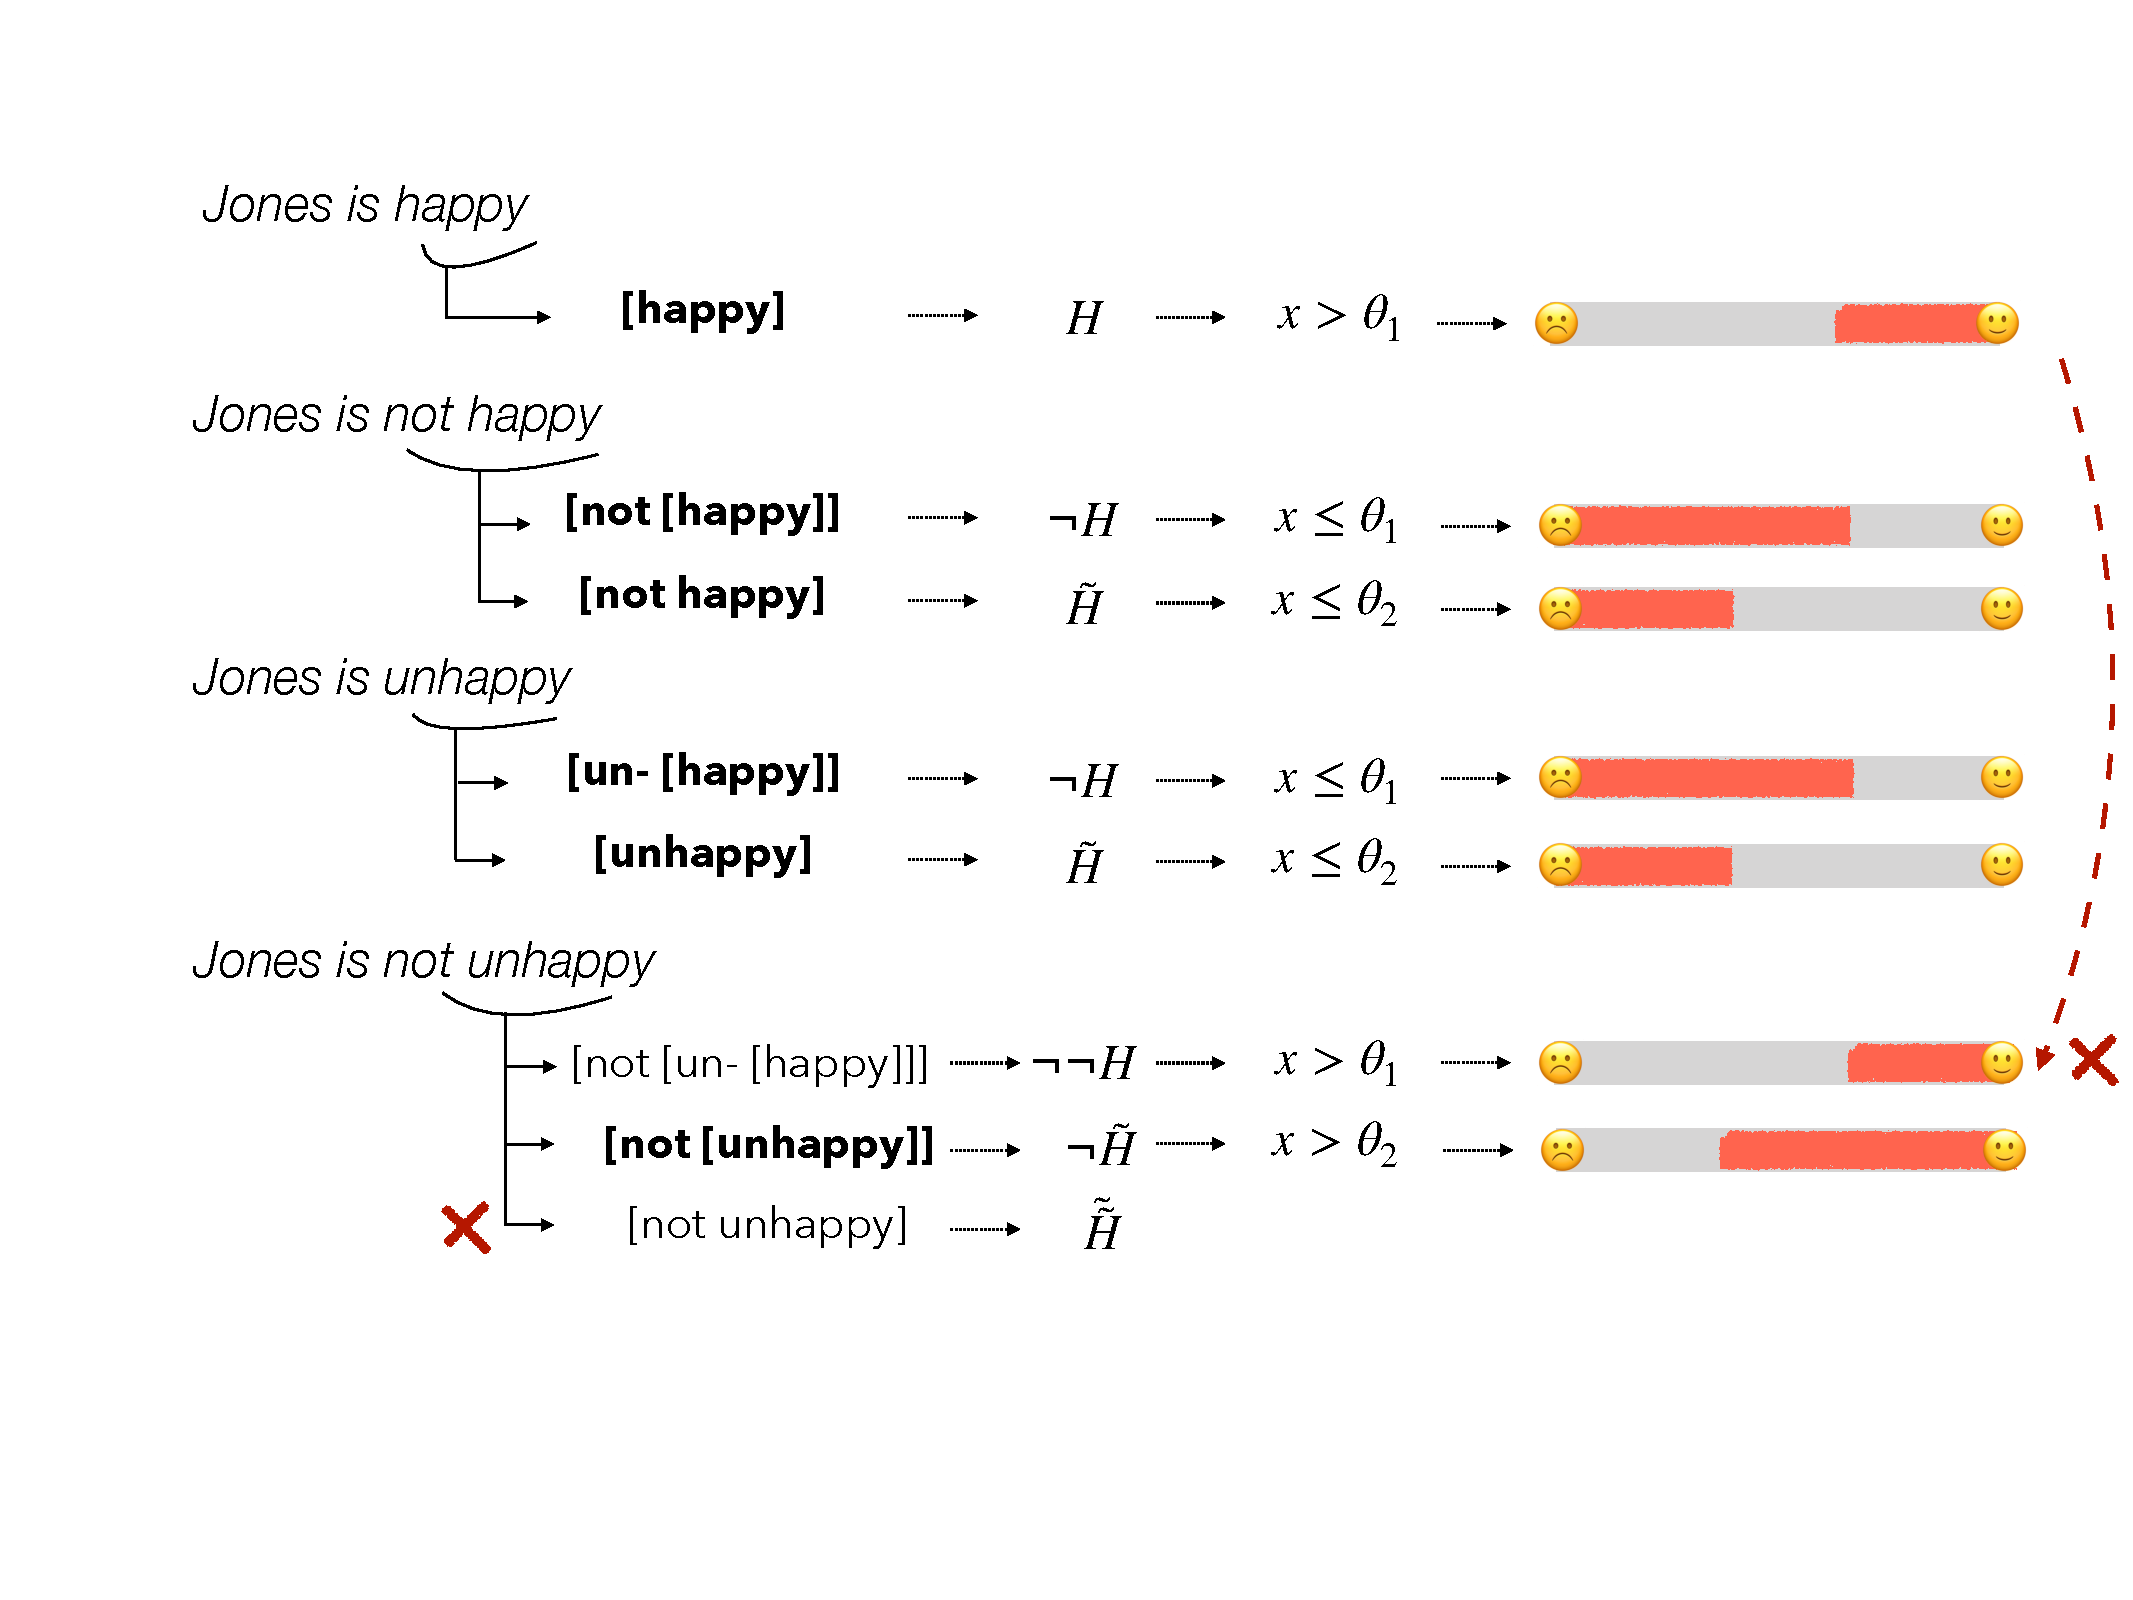
\includegraphics[width=0.8\textwidth]{figs/schematicMeanings}  
%\caption{Set of possible meanings for antonym pairs and their negations for the \ourmodel model. 
%Both ``not happy'' and ``unhappy'' could signal either contradictory $\neg H$ or contrary $\tilde{H}$ negation.
%``Not unhappy'' can signal a double contradiction  $\neg \neg H$  or a contradiction of a contrary  $ \neg \tilde{H}$. A double contrary $\tilde{\tilde{H}}$ is not logically possible. A double contradiction  $\neg \neg H$  is pragmatically unlikely, because the same meaning is expressed by just the simple positive $H$. Scales on the right denote hypothetical interpretations of the different meanings.}
%\label{fig:meanings}
%\end{figure}

%\mht{can we model this as an L2, where Lassiter adj model is modularized into $P(x \mid u, \mathcal{L})$ and we don't need to talk about thresholds?}
%\begin{align}
%P_L(x, \mathcal{L} \mid u) &\propto P_S(u \mid x, \mathcal{L}) \cdot P(x) \cdot P(\mathcal{L}) \\
%P_S(u \mid x, \mathcal{L}) &\propto \exp{(\alpha \cdot \ln {P(x \mid u, \mathcal{L})} - \text{cost}(u))} \label{eq:S1}
%\end{align}


%We hypothesize that \emph{lexical uncertainty}---uncertainty in the meaning of words---pervades even the language of logical devices, which interacts with conversational reasoning to give rise to a panoply of context-specific interpretations.
%Specifically, we posit that overt negation markers (\enquote{not}, \enquote{un-}) can convey different kinds of negation and that listeners resolve their uncertainty about the meaning in context.

The semantic distinction between contraries and contradictions (like mental representations, more broadly) cannot be observed directly, but will manifest in the mind of a listener via how they interpret natural language expressions. 
This interpretation process does not exist in a vacuum but depends upon assumptions listeners and speakers make about each other in the context of a communicative interaction \cite{Grice1975}.
We formalize this interpretation process in a computational model drawing on the tools of formal semantics and probabilistic models of pragmatics \cite{Franke2015a, Goodman2016:RSA}. 

\subsection{Formal semantic representations}

Formally, a scalar adjective $H$ (e.g., \emph{happy}) is literally true when the degree associated with that adjective \(x\) (e.g., the degree of happiness) is greater than some contextually-determined threshold \(\theta\) \cite{Kennedy2007}:
\begin{equation}
\mbox{ $[\![H]\!]$}(x, \theta): x > \theta \label{sem:pos}
\end{equation}
The intuition for this semantic representation comes from adjectives like \emph{tall}, where the underlying dimension is relatively transparent (height) and the contextually-determined threshold allows for context-sensitive interpretations (a tall boy vs. a tall building).

We study negation in the context of gradable adjectives because their degree-based semantics allows us to differentiate the meaning of negation markers when interpreted as either contradictory or contrary negation.
Contradictory negation is the truth-value swapping operation well-known from classical logic.
The contradictory opposite of $H$---$\neg H$---denotes that the actual degree of happiness is less than or equal to the contextually-relevant threshold of happiness associated with $H$: 
\begin{equation}
\mbox{ $[\![\neg H]\!]$}(x, \theta): x \leq \theta \label{sem:neg}
\end{equation}
Contrary negation, on the other hand, is characterized by a neutral middle ground.
It cannot therefore be directly anchored to the threshold $\theta$.
%; its precise denotation will depend on the further contextual features---like background conversational knowledge, statistical world knowledge etc.---which also features into the determination of the threshold $\theta$ which fixes the truth-conditions for its argument.
Contrary negation is therefore best treated as an operation that forms an entirely new predicate, with its own separate threshold $\theta'$ which merely reverses the direction on the degree-scale but is otherwise subject to the same conditions of pragmatic context resolution as $\theta$.
Concretely, contrary negation of $H$, $\tilde{H}$ introduces a new distinct threshold \(\theta'\) and assigns truth-conditions entirely independent of its argument except that it ``reverses directionality'': 
\begin{equation}
\mbox{ $[\![ \tilde{H} ]\!]$}(x, \theta'): x < \theta' \label{sem:ant}
\end{equation}

Since contradictory negation simply swaps the truth-value of the embedded predicate, this operation may be iterated, returning the original embedded predicate: $\neg \neg H = H$. Contradictions of contraries, however, denote a unique meaning by reversing the truth-value on the new predicate defined with its own threshold:

\begin{equation}
\mbox{ $[\![\neg \tilde{H}]\!]$}(x, \theta): x \geq \theta' \label{sem:negant}
\end{equation} 


Contrary negation as a predicate-forming operation discards information about the original threshold $\theta$ of the embedding predicate (e.g., if \emph{unhappy} is a contrary, it receives a different, independent threshold from that of \emph{happy}).
This fact has important consequences when we consider efficient semantic representations.
In particular, it leads to the following distributional restriction.
Let $\tilde{}$ the be contrary negation operator.
Let $\phi$ be an expression, possibly containing a negation operator. 
Since contrary negation is predicate-forming, the meaning of $\tilde{\phi}$ is independent of the (potentially compositional) meaning of $\phi$.
This means that, no matter how complex $\phi$ may be and how many of the negation operators occurring in $\phi$ are interpreted, the semantic meaning of $\tilde{\phi}$ is either that of `happy' (a single free threshold parameter giving the lower bound on the degree scale) or that of $\tilde{\textrm{`happy'}}$ (a single free threshold parameter giving the upper bound on the degree scale).
In other words, $\tilde{}$, unlike logical contradictory negation, is an operator that basically discards all information from previous compositional meaning computation.
For representational efficiency, we therefore assume that contrary negation $\tilde{}$ is distributionally restricted to not take scope over any other negation operator, including itself, as the resulting semantic meaning could always be expressed more economically. 
Consequently, $\tilde{\tilde{H}}$ is not a logical possibility \cite{Horn1989:Natural} and so, whenever a negation operator takes scope over another, the scope-taking operator cannot be contrary negation.

%Modeling contrary negation as a predicate-forming operation which discards information about the precise location of the threshold of the embedding predicate has important consequences for considerations of economic semantic representations.
%Applying predicate-forming, information-discarding contrary negation to anything else than an unmodified expression would incur spurious computation which is eventually spurious.
%We therefore assume that contrary negation $\tilde{}$ is distributionally restricted not to take scope over any other negation operator, including itself, so that $\tilde{\tilde{H}}$ is not a logical possibility \cite{Horn1989:Natural}. 


\subsection{Semantic hypotheses}

The distinction between contrary and contradictory opposition was introduced by Aristotle and we articulate a hypothesis assuming ``un-'' denotes contrary negation and ``not'' denotes contradictory negation, as defined in the section above.
We additionally articulate a hypothesis wherein only contradictory opposition exists (espoused famously by George Orwell, in the quotation at the beginning of the main text of the paper) and in which two negatives simply cancel out. 
Our \ourmodel hypothesis represents a kind of middle-ground between the two, where listeners represent a hypothesis space of possible meanings for the various negation markers (\emph{un-}, \emph{not}).
The semantic choices are summarized in Table \ref{tab:sem}.

All models assume vagueness in the meaning of the gradable adjective (e.g., \emph{happy} means the degree of happiness is greater than some uncertain, contextually-determined threshold $\theta$, inferred by the listener, described below).
We additionally compare these models to two other simpler alternatives in which there is no vagueness about the meaning of the adjective (i.e., there is a strict cut-off for someone being \emph{happy}). 
The first is an Aristotelean model that assumes lexical meanings of contraries and contradictions for \emph{un-} and \emph{not}, respectively, but which hard-codes the semantic thresholds for each:  \emph{happy} means \(>70\%\) on the happiness scale; \emph{unhappy} means \(<30\%\).
The second is a kind of a \ourmodel model without vagueness. 
This model has the same fixed threshold meanings for the adjectival utterances as the Aristotelean (no vagueness) model, but has uncertainty as to whether or not ``un'' and ``not'' convey contradictory~vs.~contrary negation. 
We omit the predictions of the logically possible \emph{George Orwell} (no vagueness) model, because they are not qualitatively different from the George Orwell model with vagueness.



\subsection{Common pragmatics core}

We embed the different semantic hypotheses as literal meanings that define a lexicon $\mathcal{L}$ to be used inside of a probabilistic model of pragmatics, wherein a pragmatic listener $L_1$ resolves the meaning of an utterance $u$ by reasoning about why a rational speaker $S_1$ would have bothered to produce said utterance.
This same pragmatics machinery is used for the Aristotelean and Orwellian hypotheses. 
A generalization of this model (described below) is used for the \ourmodel hypothesis. 

Eqs.~\ref{eq:L0}--\ref{eq:L1} describe a recursive Bayesian model in the Rational Speech Act tradition \cite{Franke2015a, Goodman2016:RSA}, 
which takes into account the vagueness of scalar adjectives using the technique proposed by \citeA{Lassiter2015} to derive thresholds \(\theta\) for interpreting vague adjectives (e.g., happy) in context:

%\vspace*{-0.5cm}

\begin{align}
L_{0}(x \mid u, \theta, \mathcal{L}) &\propto \mathcal{L}(u, x, \theta) \cdot P(x) \label{eq:L0} \\
S_{1}(u \mid x, \theta, \mathcal{L}) &\propto \exp{(\alpha \cdot \ln {L_{0}(x \mid u, \theta, \mathcal{L})} - \text{cost}(u))} \label{eq:S1}\\
L_{1}(x, \theta \mid u,  \mathcal{L}) &\propto S_{1}(u \mid x, \theta, \mathcal{L}) \cdot P(x) \cdot  P(\theta) \label{eq:L1}
\end{align}

%\vspace*{-0.5cm}

The literal listener \(L_0\) (Eq. \ref{eq:L0}) updates their prior beliefs over the degree \(P(x)\) via an utterance's literal meaning in lexicon \(\mathcal{L}\),
where \(\mathcal{L}(u, x, \theta)\) gives the truth-value of the utterance \(u\) in lexicon \(\mathcal{L}\) when applied to degree \(x\) (e.g., for $u= $ \emph{happy}, $\mathcal{L}$ returns a 1 when $x>\theta$ and a 0 when  $x\leq\theta$).
The details of this lexicon is what differs between  the Aristotelean model and the Orwellian model (and the \ourmodel model, described below).

The representation of prior beliefs $P(x)$ encodes prior expectations about the degree (e.g., how happy people are likely to be), which we assume for simplicity to be a uniform distribution over the unit-interval [0, 1].\footnote{All qualitative patterns reported replicate when this uniform prior is replaced with a Gaussian prior $\mathcal{N}(0.5, 0.5)$ and a U-shaped Beta prior: $\text{Beta}(0.5, 0.5)$.
}
The speaker (Eq.~\ref{eq:S1}) is a soft-max rational agent (with degree of rationality  $\alpha$) who aims to act in accordance with a standard, information-theoretic utility function that tracks how well an utterance conveys the speaker's intended meaning $x$ (i.e., the degree of happiness) to this literal listener---$\ln {L_{0}(x \mid u, \theta, \mathcal{L}}$)---while taking into account the cost of the utterance---$\text{cost}(u)$.
The intended meaning in this model is the value along a dimension referenced by an adjective (e.g., a degree of happiness); this intended meaning corresponds to an answer to the question (the \emph{Question Under Discussion}) ``how happy is the referent?''\footnote{
	This meaning is a special case of modeling meaning as a probability distribution over degrees of happiness (e.g., the speaker has only a rough sense of the relevant degree of happiness), in which case the speaker's utility would be a function of the KL divergence between the literal listener's prior and posterior distributions over the degree given the utterance. 
}
Following \citeA{Lassiter2015}, the prior distribution on thresholds is defined to be a uniform distribution over the unit interval $P(\theta) = \text{Uniform}(0, 1)$. 

The pragmatic listener (Eq.~\ref{eq:L1}) interprets an utterance by reasoning about two variables: the intended meaning or degree $x$ and the threshold beyond which a scalar adjective is literally true  $\theta$.  
\citeA{Lassiter2015} showed how this model can derive vague, context-sensitive interpretations of gradable adjectives (e.g., ``a tall boy''~vs.~``a tall basketball player'').
The model achieves this with relatively minimal semantic assumptions: building on the work on the work on gradable adjectives of \citeA{Kennedy2007}, the model assumes that the meaning of a gradable adjective is a threshold on the degree (e.g., \mbox{ $[\![ tall ]\!]$}= $height(x) > \theta$). 
Then, this semantics is plugged into the Rational Speech Acts model, with one addition: $\theta$ is not treated as a fixed parameter, but the pragmatic listener samples $\theta$ from a prior distribution (i.e., listener has uncertainty about theta). 
This ``uncertain threshold'' is what is able to capture the vagueness of gradable adjectives. 
Context-sensivity falls out of the prior distribution over world states $P(x)$ (a basic component in any RSA model); in this case, it is a prior distribution over degrees (e.g, prior expectations about the heights of buildings). 
\citeA{Lassiter2015} showed that the inference about the threshold actually needs to be resolved at the level of a pragmatic listener, and not at the level of a literal (semantic) listener. The reasoning behind this can be loosely described as: ``a listener who hears ‘John is tall’ reasons that a speaker would be unlikely to say ‘John is tall’ if John’s height were not sufficiently great''. 
 
The normalization in Eq.~\ref{eq:S1} implies a normalization over a set of alternative utterances (which potentially differ in their cost). 
We assume in our models that the set of alternative utterances is the positive adjective, the antonym, and their corresponding particle negations (e.g., happy, unhappy, not happy, not unhappy). 
We further assume the cost of morphological negation is less than the cost of particle negation (i.e., $cost(un) < cost(not)$) and that costs are additive (i.e., $cost(not\text{ }un) = cost(un) + cost(not)$), though we examine model predictions under different assumptions of cost below. 
%We assume that negating morphological antonyms is a possibility (i.e., \emph{not un-} is a possible utterance) though there is no corresponding morphological antonym of a particle negation (i.e., there is no \emph{un- not}). 

\subsubsection{Orwellian model}

The Orwellian model assumes that both \emph{unhappy} and \emph{not happy} are logical contradictions of the embedded predicate \emph{happy}.
These meanings amount to stipulating an upper-bound on the degrees of happiness (Equation \ref{sem:neg}), where that threshold is the same threshold as for \emph{happy} (Table \ref{tab:sem}).
Thus, there is only one threshold $\theta$ in this model. 

The pragmatics machinery, in this case, does nothing particularly notable.
As one might expect from the semantics alone, the \emph{George Orwell} semantics is too constraining to distinguish different kinds of negation, and a double negation like \emph{not unhappy} returns the same distribution as the positive adjective (\emph{happy}; Figure \ref{fig:modelPredictions}).

\subsubsection{Aristotelean model}

The Aristotelean model assumes that the \emph{happy} and \emph{unhappy} are contraries, which each gets assigned their own truth conditional threshold (e.g., $\theta$ and $\theta'$). Thus, instead of the pragmatic listener defined by Equation \ref{eq:L1}, we have: 
%
\begin{align}
L_{1}(x, \theta, \theta' \mid u,  \mathcal{L}) &\propto S_{1}(u \mid x, \theta, \theta', \mathcal{L}) \cdot P(x) \cdot  P(\theta)  \cdot  P(\theta') \label{eq:L1aris}
\end{align}
%
Both thresholds are drawn from uniform prior distributions. The only thing that distinguishes the thresholds is that one corresponds to a lower-bound (for \emph{happy}; Eq.~\ref{sem:pos}) and the other corresponds to an upper bound (for \emph{unhappy}; Eq.~\ref{sem:ant}). 

The thresholds are determined via pragmatic reasoning in the very same way as they are for the simple case of a positive adjective: ``happy'' ends up meaning \emph{significantly happier than you might expect} and its antonym (``unhappy'') means \emph{significantly less happy that you might expect}. 
The contradictory negations of the polar contraries then pick out the complement set of what is referred to by the embedded adjectival predicate, but because of pragmatic competition with the other alternative utterances, the negated utterances end up carving up the intermediate zone of degrees. 

This is a testament to the productive nature of the RSA framework and the \citeA{Lassiter2015} adjectives model in particular that the model is able to predict the intuitive ordering expressed by \citeA{Krifka2007:Negated-antonyms}: \emph{unhappy} $<$ \emph{not happy} $<$ \emph{not unhappy} $<$ \emph{happy}, with \emph{not unhappy} receiving a slightly positive interpretation (Figure \ref{fig:modelPredictions}).
The model achieves this with very lean semantic assumptions about the meanings (e.g., we do not even stipulate $\theta'$ < $\theta$; that the threshold for unhappy is less than the threshold for happy, but the model reasons that this would be communicatively useful way of setting the thresholds; Aristotle No Vagueness).

We also explore the predictions of a contraries and contradictions model where the thresholds for \emph{happy} and \emph{unhappy} are fixed. This model corresponds to a Vanilla RSA model (i.e., no reasoning about thresholds). 
This model is also too rigid to produce the intuitive ordering. 
The model reasons that \emph{not unhappy} does not communicate the same region of the space as \emph{happy}; instead, the model restricts its interpretation to the neutral zone (i.e., \emph{not unhappy but not happy}); the same logic plays out for \emph{not happy}, which receives the same neutral-feelings interpretation  (Figure \ref{fig:modelPredictions}; Aristotle No Vagueness).


%, and the likelihood \(S_1(u \mid x, \theta, \mathcal{L})\) that a cooperative information-maximizing speaker would utter the adjective given a degree \(x\), threshold \(\theta\), and lexicon \(\mathcal{L}\).
%The speaker model \(S_1\) (Eq.\ref{eq:S1}) describes an approximately rational agent (with degree of rationality \(\alpha\)) trying to inform a naive listener \(L_0\) about the degree \(x\).

%\begin{figure}
%\centering
%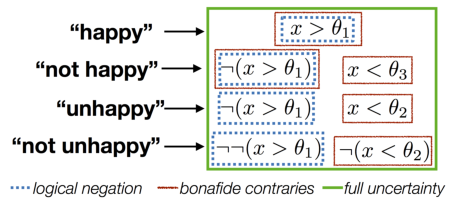
\includegraphics{figs/lexicon-model-1.pdf}
%\caption{\label{fig:lexicon-model}Space of possible meanings in the lexicon prior for the \emph{logical negation}, \emph{bonafide contraries}, and the full \emph{\ourmodel} models.}
%\end{figure}

\begin{table}[t]
\centering
\begingroup\fontsize{10pt}{11pt}\selectfont
\begin{tabularx}{0.9\textwidth}{l|c|c|c}
\toprule
Model Name                      & “happy”        & “un-”                            & “not ”                           \\ \midrule% & Description\\ \midrule
Aristotle no Vagueness                                                    & $x > 0.7$      & $x < 0.3$                        & $x < 0.7$                        \\% & Hard-coded contraries and contradictions \\
Aristotle with Vagueness                                 & $x > \theta$ & $x  < \theta'$                  & $x \leq \theta$                   \\% & Contraries and Contradictions \\
George Orwell with Vagueness                                                 & $x > \theta$   & $x < \theta$                     & $x < \theta$                     \\% & Only Contradictions \\
%Vanilla Lexical Uncertainty & No       & In Principle                         & $x > 0.7 $ & $x  < 0.3$ or   $x  < 0.7$              &  $x  < 0.3$ or   $x  < 0.7$                       \\% & Contraries and Contradictions \\
\ourmodel  no Vagueness                                & $x > 0.7$ & $x  < 0.3$ or $x \leq 0.7$ & $x  < 0.3$ or $x \leq 0.7$ \\ %& Uncertain how “un” and “not” correspond with contrary vs. contradictory negation \\
\ourmodel   with Vagueness                               & $x > \theta$ & $x  < \theta'$ or $x \leq \theta$ & $x  < \theta'$ or $x \leq \theta$ \\ %& Uncertain how “un” and “not” correspond with contrary vs. contradictory negation \\
\bottomrule
\end{tabularx}
\endgroup
\caption{Space of alternative models and the literal meanings they ascribe to adjectival utterances. When the literal meaning makes reference to a $\theta$ variable, that indicates that this variable is not fixed \emph{a priori} but is inferred by the listener model.}
\label{tab:sem}
\end{table}



%Second, we compare to the Vague RSA model of \citeA{Lassiter2015}, assuming that all negation markers entail contradictory negation (the \emph{logical negation} or \emph{George Orwell} model).
%Finally, we construct a \emph{bonafide contraries} model, building on \citeA{Lassiter2015}'s Vague RSA model by assuming morphological antonyms (\emph{un-}) convey contrary negation (e.g., \emph{unhappy} is to \emph{happy} how \emph{short} is to \emph{tall}) while the negation particular \emph{not} conveys contradictory negation.
%Finally, we construct fixed-threshold version of the \ourmodel model: this model is a lexical uncertainty model in the style of \citeA{Bergen2016}, which differs from our \ourmodel model only in its treatment of the semantics of the adjective as fixed as opposed to vague. 




\begin{figure}[t]
\centering 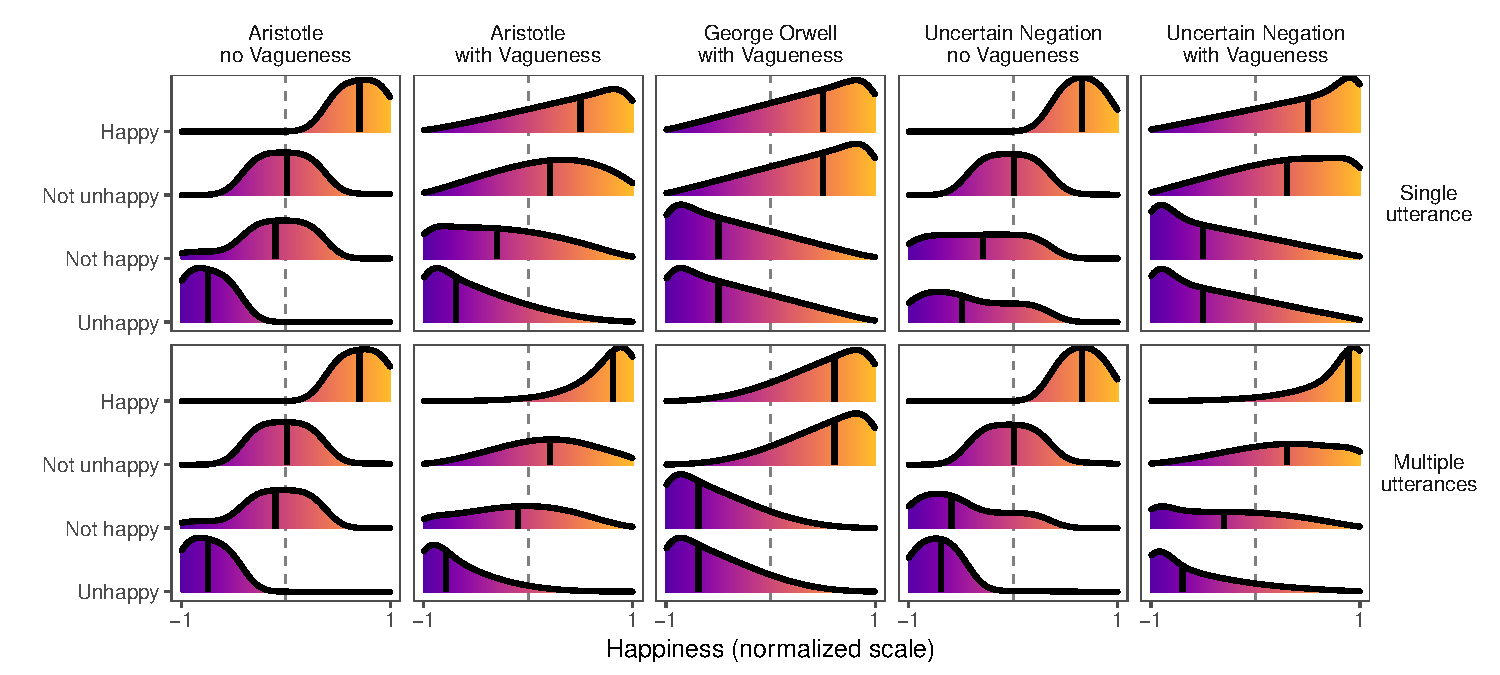
\includegraphics{figs/alternativeModels_all5_fine_dists.pdf} 
\caption{Model predictions for interpretations of antonym pairs and their negations. The \emph{\ourmodel} model shows unique qualitative patterns, exhibiting qualities of both the \emph{George Orwell} and \emph{Bonafide Contraries} models when the utterances are presented in isolation (Single Utterance condition); when utterances are presented in the same context (Multiple Utterances condition), \emph{\ourmodel} makes predictions similar to the \emph{Bonafide Contraries} model. Model predictions use the following minimally assumptive model parameters: $P(x) = \text{Uniform}(0, 1); \alpha = 1; \text{cost}(\mathit{un}) = 2; \text{cost}(\mathit{not}) = 3$.}.\label{fig:modelPredictions}
\end{figure}


\subsubsection{Flexible Negation model}

We extend the Aristotelean model (Eq.~\ref{eq:L1aris}) by introducing uncertainty into the pragmatic listener about how their interlocutor (speaker $S_1$) uses negation markers to convey contradictory~vs.~contrary negations \cite{Bergen2016}.
This uncertainty takes the form of a prior distribution over lexica: $P(\mathcal{L})$.

\begin{align}
L_{1}(x, [\theta], \mathcal{L} \mid u) &\propto S_{1}(u \mid x, [\theta], \mathcal{L}) \cdot P(x) \cdot  P([\theta]) \cdot P(\mathcal{L}) \label{eq:L1a}
\end{align}
% 
where $[\theta]$ could represent a vector of thresholds (e.g., $[\theta, \theta']$), if the lexicon $\mathcal{L}$ contains contraries.
The other components of the model ($S_1$ and $L_0$) are the same as Eqs.~\ref{eq:L0} \& \ref{eq:S1}.

\paragraph{Lexicon prior}
%
We assume a relatively symmetric hypothesis space of lexica, wherein either \emph{un-} or \emph{not} could express contraries or contradictions. 
This leads to four logically possible lexica governing the meanings of \emph{not} and \emph{un-}: both are contradictory negation (George Orwell), \emph{un-} is a contrary and \emph{not} is a contradiction (Aristotle), \emph{not} is a contrary and \emph{un-} is a contradiction, and both are contraries. 
We assume a uniform prior over lexica (each has probability 0.25), though we discuss relaxing this constraint below. 

%The logical foundations of contrary negation impose certain constraints on lexica, however.


The distributional restriction for contraries (described in the Formal Semantic Representations section above) introduces a complication when dealing with negated morphological antonyms (\emph{not un-})  under lexica in which \emph{not} is a contrary. 
% when (the outer negation) \emph{not} is a contrary because 
 The distributional restriction would render this utterance impossible for this kind of lexicon.
We thus constrain the lexicon in these cases to remove the \emph{not un-} utterance from lexica involving \emph{not} as a contrary. 
We implemented this restriction by making the \emph{not un-} utterance vacuously true for lexica wherein \emph{not} is a contrary.\footnote{We decide to operationalize the restriction via a semantic vacuity as opposed to simply removing the utterance from the lexicon because the latter results in certain states $x$ (i.e., degrees, e.g., degrees of happiness) being unreferrable by all utterances under certain values of the thresholds (i.e., under certain, logically possible regimes of threshold values, all utterances are false for certain states). This leaves the model mathematically undefined and unanalyzable.}

\paragraph{Model predictions}%
With these assumptions, the model reasons much like the Aristotelean model about the thresholds for positive adjectives and contraries, but the uncertainty about whether \emph{not} or \emph{un-} (or neither) conveys contrary opposition leads to a key quasi-ordinal prediction:The model does not differentiate \emph{unhappy} (antonyms) from \emph{not happy} (negated positives), as \citeA{Jespersen1917:Negation} and \citeA{Blutner2004:pragmatics} surmised.
At the same time, upon hearing \emph{not unhappy}, the \emph{\ourmodel} model reasons that a truly compositional \(\neg \neg \textit{happy}\) is implausible because the speaker could have just said the simpler \emph{happy} and interprets the utterance as signaling a slightly positive state (Figure \ref{fig:modelPredictions}).
%This pattern of judgments is uniquely predicted by the \emph{\ourmodel} model.
%The \emph{bonafide contraries} model also yields interpretations of negated antonyms as slightly positive, but predicts that \enquote{unhappy} (morphological antonym) signals a more negative state than \enquote{not happy} (negated positive).
%The \emph{logical negation} model does not differentiate between negated antonyms and positives, nor between negated positives and antonyms.

\subsubsection{Modeling the ``multiple utterances'' condition}

The \emph{\ourmodel} model's predictions are derived by reasoning about which lexicon best explains a speaker's utterance (Fig.\(\thinspace\)\ref{fig:modelPredictions}, \emph{single utterance}).
Hearing multiple utterances by the same speaker, however, can provide the listener with more information about the speaker's lexicon, as in \citeA{Krifka2007:Negated-antonyms}'s example above (``I wasn't unhappy, just not happy''). 

The formal modeling approach we take here naturally allows for this extension by simply providing \(L_1\) with multiple adjective phrases; we condition each model on the observation of a speaker using all four adjective alternatives $u'$ to describe different referents $x'$ (e.g., \emph{Sue is happy. Steve is not happy. Bill is unhappy. Barb is not unhappy.}; Figure \ref{fig:modelPredictions}, \emph{multiple utterances}).

\begin{align}
L_{1}([x], [\theta], \mathcal{L} \mid [u]) &\propto \prod_{{u', x'} \in \{[x],[u]\}} S_{1}(u' \mid x', [\theta], \mathcal{L}) \cdot P(x') \cdot  P([\theta]) \cdot P(\mathcal{L}) \label{eq:L1multi}
\end{align}


%Hearing multiple utterances has no effect on the Vanilla RSA model because it ascribes no uncertainty in meaning to the linguistic messages.
All models with vagueness in the predicates derive more extreme differences in interpretations between utterances that could have different meanings (e.g., the difference between \emph{happy} and \emph{not unhappy} for \emph{Aristotle} is greater when it hears multiple utterances).
This inference results from the fact that the listener has more evidence that the speaker intends different meanings for the different linguistic messages by virtue of the fact that the speaker used different messages.
Crucially, this inference results in the \emph{\ourmodel} model predicting an interpretative difference between \emph{unhappy} and \emph{not happy}, wherein \emph{unhappy} is more sad than \emph{not happy}, producing the ordering hypothesized by \citeA{Krifka2007:Negated-antonyms} when both are used in the same context.
It is this model prediction from which we derive the prediction for an interaction between morphological vs. negated positives X single vs. multiple utterances. 
%All models have more extreme interpretations when they condition on multiple utterances.


\subsubsection{Symmetry breaking in the \ourmodel model}
%
The Flexible Negation model is able to predict that (when heard in the same context) \emph{unhappy} is more negative than \emph{not happy}.
This prediction is a result of the cost asymmetry between \emph{un} and \emph{not}, and without it, \ourmodel does not interpret the two differently in the multiple utterances context (Figure \ref{fig:flexNeg_variants}, left two facets).

The symmetry of morphological vs. particle negation can be broken, however, by another source in the model: the structure of the lexicon prior. 
In particular, if we interpret the distributional restriction on contraries (described above) as not only constraining the space of possible meanings given certain lexica (i.e., rendering \emph{not unhappy} meaningless in certain lexica) as we previously described, but constraining the space of lexica itself, then the ``both contraries'' lexicon would be rendered invalid (or perhaps more generously, lower prior probability). 
That is, the lexicon prior would include the possibility that either \emph{not} or \emph{un-} are contraries or that they are both contradictions,  but they cannot both be contraries. 
%which could be motivated by the distributional restriction imposed by the fact that contraries cannot iterate, results in symmetry-breaking even when there are symmetric costs between morphology and particle negation. 
In this version of the model, we also make the assumption that under the lexicon where ``not'' is a contrary, the utterance  ``not unhappy'' is not vacuous (as previously assumed) but that``not'' can be coerced to be a contradiction when it appears as the second negation in an utterance. 
With these alternative assumptions about the structure of lexicon prior, the symmetry between ``not'' and ``un-'' can be broken even with symmetric costs (Figure \ref{fig:flexNeg_variants} right facets). 

\begin{figure}[t]
\centering 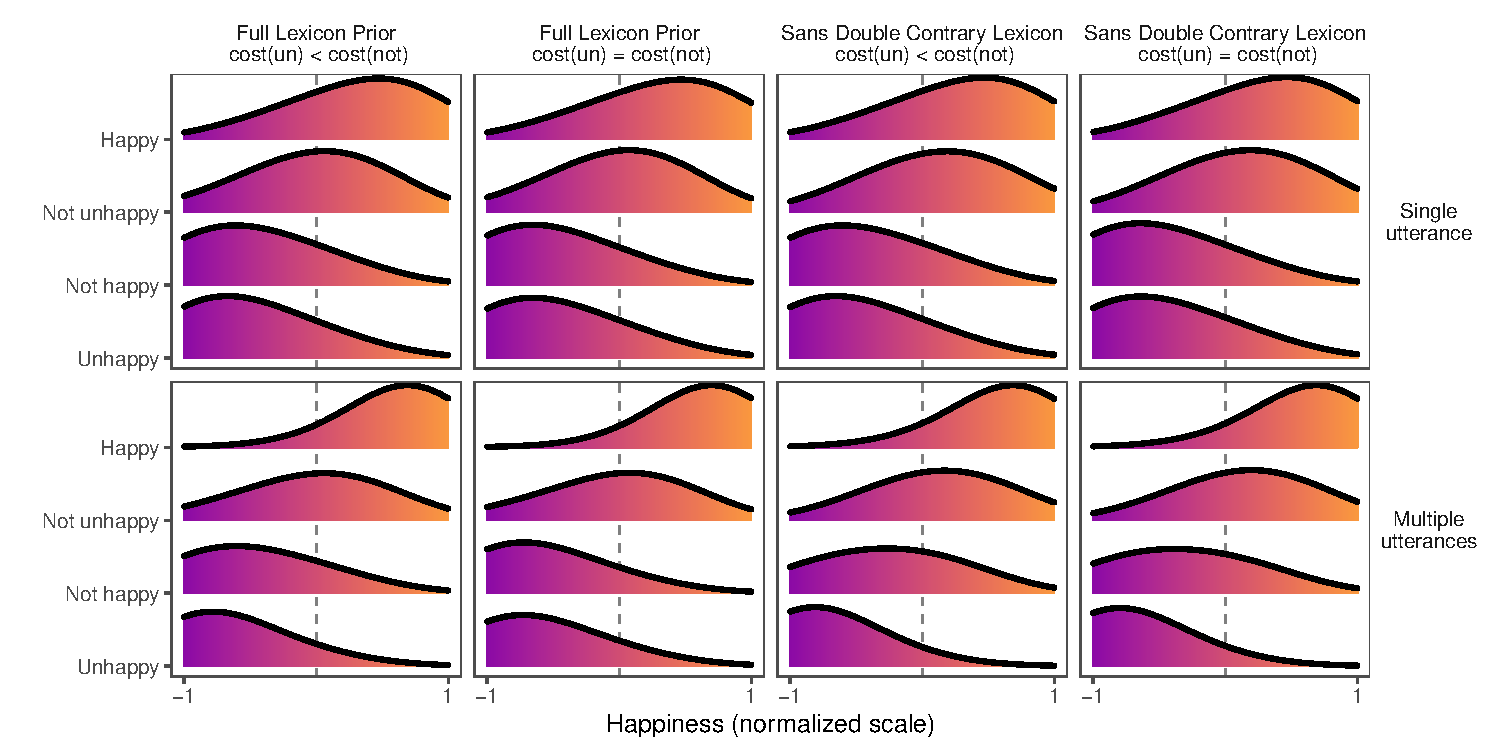
\includegraphics{figs/flexNeg_SI.pdf} 
\caption{Symmetry breaking for Flexible Negation model can be driven by cost difference (cost(un) $<$ cost(not)) (left-most facet) or by removing the ``double contrary'' lexicon from the hypothesis space of Lexica (with symmetric costs) (right two-facets).}.\label{fig:flexNeg_variants}
\end{figure}

%We assume that negation created by morphology (e.g., ``un-'' + happy) adds cost to the utterance as does creating a negation using the particle ``not'', and that the cost of ``un-'' is less than the cost of ``not''.
%The fact that the \ourmodel model's qualitative predictions are sensitive to the exact values of the parameters. 

Thus the symmetry between ``not'' and ``un-'' in the \ourmodel model can be broken by either cost asymmetries or by the structure of the lexicon prior.
Our goal here is not to argue for a particular form of this model.
Our goal is to show, under intuitively plausible parameter values consistent with the literature using Rational Speech Act models, that the \ourmodel model has the capacity to the make the predictions we describe; none of the alternative semantic models we articulate have the capacity to make the unique predictions of the \ourmodel model.
The cost-based predictions are invariant to the exact values of cost so long as $\text{cost}(un) \leq \text{cost}(not)$ and $\alpha$ is relatively small. 

%The first of these alternatives is a ``Vanilla RSA'' model which has neither lexical uncertainty about negation nor vagueness in the meaning of the adjective \cite{Frank2012}; we assume for this model an Aristotelean analysis of the negation markers (\emph{not} means contradiction; \emph{un-} means contrary) operating over fixed threshold meanings:
%We call this model \emph{Aristotle no vagueness}.




%According to the \ourmodel model, listeners are uncertain about how \emph{not} and \emph{un-} map onto these logical meanings, and therefore negated positives like \emph{not happy} and morphological antonyms like \emph{unhappy} could in principle take either meaning. 
%The hypothesis space of meanings for negated antonyms like \emph{not unhappy}, however, is constrained by the fact that contraries do not iterate; thus, negated antonyms either correspond to a double application of contradictory negation or a contradiction of a contrary.
%\mht{there is a still a question of here of what to do with ``not un-'' when un- is contradiction and not is contrary. V1: commutative -- flip order of un- and not and get a contradiction of contrary. V2: order-dependent but outer ``not'' always takes contradiction regardless if there is an inner negation}.
% \footnote{``not un-H'' can then be either \(\neg \neg H\) or \(\neg (\tilde{H})\). Cashing these meanings out in terms of scalar adjectives, the order of operations need not matter: \(\neg (\tilde{H})\) $= \tilde{(\neg H)}$ , because both imply two sign-changes and one tokenization of a new threshold.}




%The act of producing a negated antonym (\enquote{not unhappy}) can then act as a signal towards the kinds of oppositions that the speaker had in mind (e.g., that the speaker intends to convey a contradictory negation of a contrary opposite).
%\mht{i think this point could be moved to a model implementation appendix or footnote}

%\red{Contradictory opposition can be iterated (\(\neg \neg Hx\)) but contrary opposition cannot \cite{Horn1989:Natural}.
%As a result, a single negative (\enquote{not happy} and \enquote{unhappy}) can mean either \(\neg happy\) or \(\tilde{happy}\), while double negatives (\enquote{not unhappy}) may mean \(\neg \neg happy\) or \(\neg \tilde{happy}\) (Fig.\(\thinspace\)\ref{fig:lexicon-model}).}

%In order to generate predictions, 


\subsection{Alternative pragmatic hypotheses}

Here we describe two families of alternative pragmatic hypotheses. Both of these use the Aristotelean semantics. 
The first alternative is a version of a model proposed by \citeA{Horn1989:Natural} (Ch.~5), which was developed to explain why the Aristotelean-hypothesis contradictory meaning of ``not'' gets strengthened to a polar-opposite contrary.
The second is a model that treats certain utterances as more likely to be produced by speakers when a certain \emph{Question Under Discussion} is being addressed; a listener then jointly infers the QUD along with the degree that is conveyed by the adjectival utterance.
We articulate these models in order the demonstrate the difficulty of predicting the empirical patterns of data we observe. 
We think that both of these proposals are plausible and could be further developed in future research.


\subsubsection{The effect of a mid-point denoting alternative (inspired by Horn, 1989)}

The idea that negated positives (``not happy'') and morphological antonyms (``unhappy'') can be interpreted similarly dates back at least to \citeA{Horn1989:Natural}. 
The mechanism proposed for why these get interpreted similarly is known as \emph{negative strengthening}, where pragmatic reasoning strengthens the negated positive (``not happy'') to be interpreted more similarly to the antonym.
Roughly, a listener who hears ``William is not happy'' might wonder why the speaker would go to the trouble of telling them William is ``not happy'' if the speaker didn’t believe that William’s happiness was relatively low.
This reasoning, it is supposed, can all unfold within the semantics of Aristotle, where ``not'' indicates a contradiction and ``un'' a contrary. 
Without a formal model, however, it is not really clear what components  are necessary for this computation and if the components would really add up in the right way to produce the symmetry of interpretation between ``not happy'' and ``unhappy'' while also maintaining the asymmetry between ``not unhappy'' and ``happy''.

Here, we take a first attempt at modifying the Aristotelean model to encoded reasoning more in line with the idea of negative strengthening. 
In particular, we explore the effects of including a mid-point denoting alternative utterance like ``fine/ok/content''. 
We formalize the mid-point alternative using an interval semantics, where the utterance is true if the degree of happiness is within a certain range $\theta^*$ of the midpoint (assumed to be 0.5). The formal semantics of the midpoint denoting alternative are given by: 

\begin{equation}
\mbox{ $[\![\text{fine}]\!]$}(x, \theta^*): 0.5-  \theta^* < x < 0.5  + \theta^* \label{sem:fine}
\end{equation} 

We add this semantics to the Aristotelean lexicon and embed it within the same pragmatics model given by Equation \ref{eq:L1aris}.
The listener now jointly infers the midpoint interval width ($\theta^*$) using the same pragmatic machinery as we do for other adjective threshold variables.\footnote{The prior distribution for $\theta^*$ cannot be defined over the range [0, 1] as we did for the other threshold variables. Instead, the prior for $\theta^*$ is $P(\theta^*) = \text{Uniform}(0, 0.5)$.}
We test this modified Aristotelean model under two different sets of assumptions: (1) including ``fine'' as an alternative utterance for all utterances and (2) including  ``fine''  as an alternative only for the negated positive adjective (“not happy”). 
We thought that (2) would give the highest chance of success, though the model is itself
question-begging (why should only ``not happy'' have the neutral alternative, but not the others?).  
The results for a range of parameter values (speaker optimality and cost) are shown in Figure \ref{fig:horn}. 

We find that the inclusion of a mid-point denoting alternative like ``fine'', does indeed have
the desired effect on ``not happy,'' but it also affects the interpretation of other
expressions in undesirable ways.
In the first version of the model (``fine'' added to alternative set for interpreting all utterances), the midpoint alternative affects both of the negated utterances in a relatively symmetric way.
That is, the more that ``fine'' pushes ``not happy'' into the unhappy region of the space, it also pushes ``not unhappy'' into the ``happy'' region of the space. 

\begin{figure}[t]
\centering 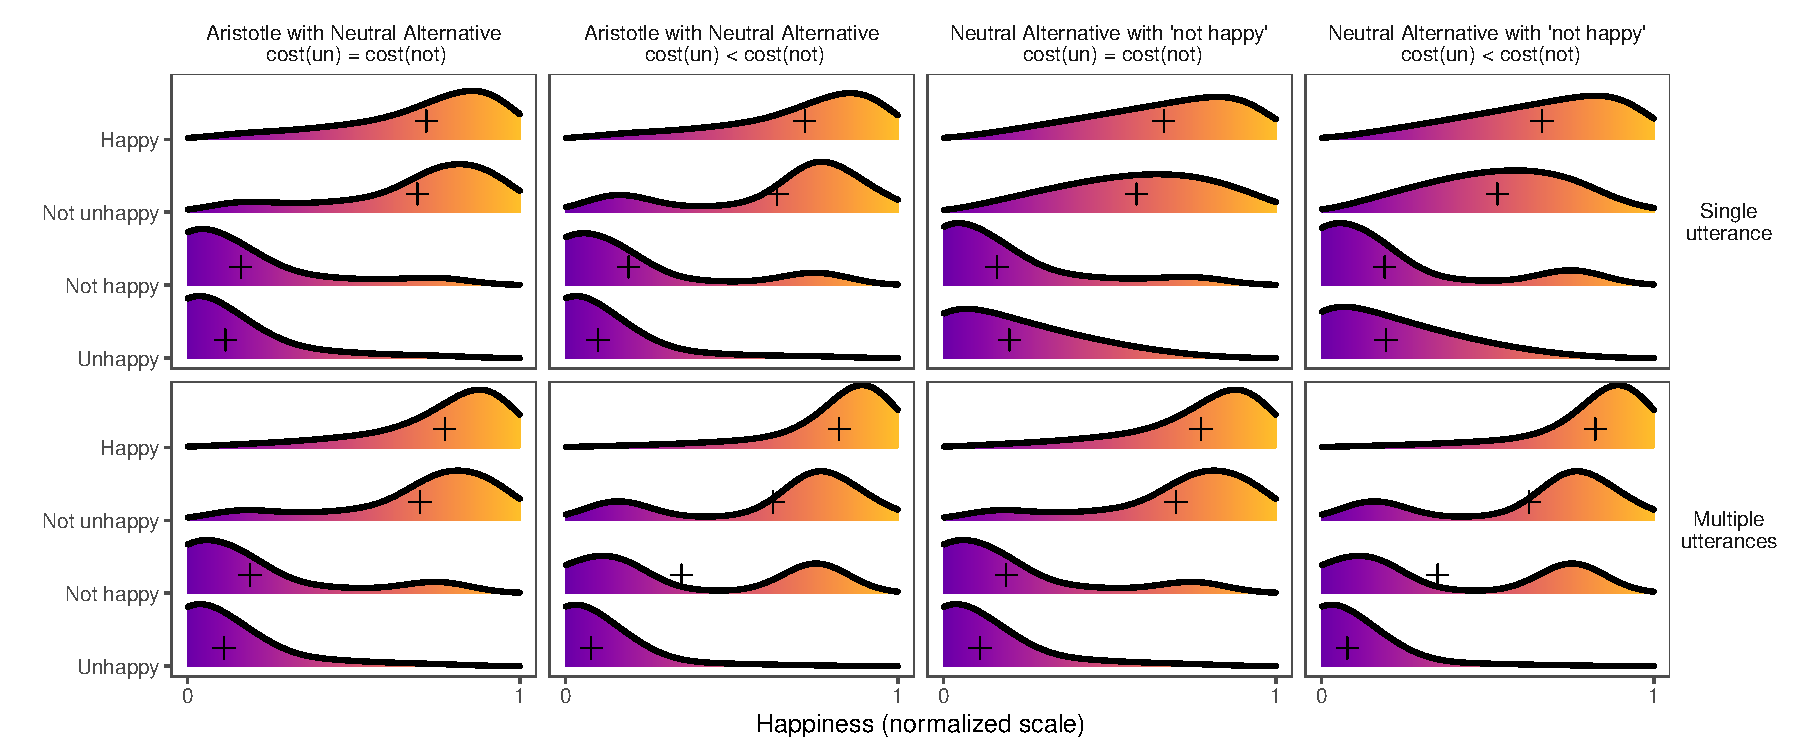
\includegraphics{figs/horn_SI.pdf} 
\caption{The effect of a mid-point denoting alternative, inspired by Horn (1989). Models use the Aristotelean lexicon with a neutral, mid-point denoting alternative utterance (``fine''). Left-most facets (``Aristotle + Neutral Utterance'') show a model where  the mid-point alternative is always an option for the speaker. The neutral utterance drives the interpretation of ``not happy'' closer to that of ``unhappy'', while also driving ``not unhappy'' closer to ``happy''. Right-most facets (``Neutral  with `not happy''') show a model where the mid-point utterance is an alternative utterance only with ``not happy''. As a result of the threshold inference that must occur for gradable adjectives, the mid-point utterance introduces a bimodality into the interpretation of ``not happy'', where ``not happy'' could mean a positive degree of happiness.}.\label{fig:horn}
\end{figure}


This symmetry can be broken by removing ``fine'' as an alternative utterance for ``not
unhappy'' (in a post-hoc, question-begging way), but the interval utterance brings further
problems, which result from the basic premise that thresholds for both contraries (``unhappy'',
``happy'') as well as the interval utterance (``fine'') are \emph{a priori} uncertain (to account for the vagueness, see above). 
In particular, the competition with the midpoint alternative introduces a bimodality into the interpretation for ``not happy'', wherein some probability is placed in the positive region of the space (i.e, \emph{rather happy}).
This second mode emerges because it is possible for the threshold for ``happy'' to be very high and the interval denoting ``fine'' relatively narrow; in this case, there is room in between ``happy'' and ``fine'' where ``not happy'' is the best utterance (an interpretation like: \emph{not extremely happy but also not just fine}, perhaps conveyed with prosodic stress ``I'm not HAPPY''). 

This kind of bimodal interpretation is not necessarily wrong. Multimodality is a feature in our empirical data and there are a variety of interpretations of antonyms and their negations having to do with prosodic stress and issues concerning the Question Under Discussion (see below). 
The presence of multimodality in the interpretations of the revised Aristotelean model, however, could be more artifactual than explanatory. 
We might prefer, from a theoretical perspective, to explain this kind of multimodality via other mechanisms (e.g., politeness, an idea also suggested by \citeNP{Horn1989:Natural}). 

To conclude, we believe the idea of negative strengthening of the negated positive adjective is intuitive, but the most natural way of implementing this phenomenon does not easily explain the empirically observed data. We believe that the jury is out as to how to implement the Aristotle+Horn approach in a manner consistent with our empirical findings. 


\subsubsection{QUD-based models}

The interpretation of linguistic messages often hinges critically on contextually available alternative utterances that can define the ``Question Under Discussion'' (QUD), the implicit communicative goal that the speaker is trying to achieve \cite{roberts2012information, beaver2017questions}. 
For example, if a speaker asks, ``Is Mary unhappy?'' and you reply, ``No, she's not unhappy'', that could imply something different than if the speaker simply asked ``How is Mary doing?'' and you replied the same way.
In particular, expressions involving particle negation (``not'') might be preferentially deployed when addressing Polar (yes/no) QUDs (e.g., ``Is Mary unhappy?'').
In all of  our models, we have assumed a neutral ``state'' QUD (analogous to the second question: ``How is Mary doing?''). 
Stress can often modulate the QUD (e.g., ``She's not UNhappy''), yet since we do not have control over the prosodic stress placed on utterances in our text-based study, it remains a possibility that some kind of QUD-inference could be occurring that would lead to the pattern of results we observe in our experiments. 

Formalizing the influence of QUDs on language understanding is a general problem in language understanding that we cannot fully address in this paper. 
The influence of a particular QUD on reasoning with a particular probabilistic model of pragmatic reasoning is, however, a well-defined relationship that we can interrogate \cite{kao2014nonliteral, hawkins2015you, hawkins_goodman_2017}. 
A QUD is a projection function that collapses irrelevant dimensions of a state onto the relevant dimensions defined by the QUD. 
For example, a polar QUD such as ``Is Mary unhappy?'' would divide the continuous state space of Mary's degrees of happiness $x \in [0, 1]$  (a real number between 0 and 1) into a binarized state space where there are only two states $Q(x) = \{\texttt{T}, \texttt{F}\}$ corresponding to the affirmative and negative answers to the question (\emph{she is unhappy}, \emph{she is not unhappy}). 
More precisely, the projected state space corresponding to the Polar QUD corresponds to whether Mary's degree of happiness is above or below the truth-conditional threshold $\theta$:  $Q(x, \theta) = \{x > \theta, x \leq \theta\}$.  
We assume there are three possible QUDs: $Q_{state}(x) = x$, $Q_{happy}(x, \theta) = x > \theta$, $Q_{unhappy}(x, \theta') = x< \theta'$. We describe both $Q_{happy}$ and $Q_{unhappy}$ as ``Polar QUDs'' or $Q = \text{Polar}$. 
 
To understand how QUDs might influence the interpretation of antonym pairs and their negations, we formalize a generative model of speaker utterances based on different QUDs and describe how a listener should invert this generative model to simultaneously infer the QUD as well as report on the state (e.g., the degree of happiness). 
Our hope is that this model will serve as a starting point for future research on the influence of QUDs on negation interpretation. 
The QUD inference model extension of the Aristotelean semantics model is given by: 
%
\begin{align}
L_{0}(\mathcal{Q}(x) \mid u, \theta, \mathcal{L}_{aristotle}, \mathcal{Q}) &\propto \mathcal{L}_{aristotle}(u, x, \theta) \cdot P(x) \label{eq:L0q} \\
S_{1}(u \mid x, \theta, \mathcal{L}_{aristotle}, \mathcal{Q}) &\propto \exp{(\alpha \cdot \ln {L_{0}(\mathcal{Q}(x) \mid u, \theta, \mathcal{L}_{aristotle}, \mathcal{Q})} - \text{cost}(u))} \label{eq:S1q}\\
L_{1}(x, \theta, \mathcal{Q} \mid u,  \mathcal{L}_{aristotle}) &\propto S_{1}(u \mid x, \theta, \mathcal{L}_{aristotle}, \mathcal{Q}) \cdot P(\mathcal{Q}) \cdot P(x) \cdot  P(\theta) \label{eq:L1q}
\end{align}
%
This model assumes that if a speaker is trying to address a polar QUD, they will only say ``yes'' or ``no'' (e.g., to address the question ``Is John happy?'', the speaker will say ``happy'' or ``not happy''). 
The pragmatic listener reasons about the QUD by considering this model of speaker behavior; thus, when they hear ``John is not happy'', they should be more likely to believe the utterance was in response to a polar QUD (\emph{is John happy?}). 
This model is styled after the QUD inference model introduced by \citeA{kao2014nonliteral} and further developed by \citeA{hawkins2015you, hawkins_goodman_2017}.
We assume the neutral State QUD and Polar QUDs are equiprobable \emph{a priori}, with the probability mass of Polar QUDs equally divided between $Q_{happy}$ and $Q_{unhappy}$ (i.e,. the prior distribution over QUDs is $\{\text{support}: [Q_{state}, Q_{happy}, Q_{unhappy}], \text{probabilities}: [0.5, 0.25, 0.25]\}$.

The inferences from this model in the single utterance condition are shown in Figure \ref{fig:qud}. 
This model of QUD inference does indeed bring the interpretation of ``not happy'' closer in line with that of ``unhappy'', but it does so at the cost of making the interpretation of ``not unhappy'' almost identical with that of ``happy''. 
The reason comes down to the inference about the QUD. It is true that, given a polar QUD, the interpretation of a negation will be similar to that of the antonym (and the negated antonym will be similar to the positive adjective). 
The issue is that the evidence that a listener would use to infer a Polar QUD (i.e., the presence of the negation particle ``not'') is strictly stronger when it appears with the antonym created by morphology, because of the additive nature of cost. ``Not unhappy'' is always the costliest utterance in the set of alternatives, and given this utterance, the listener places almost 99\% probability mass on this utterance being an answer to the Polar QUD (\emph{is Mary unhappy?}). 
Given the utterance ``not happy'', the listener also more strongly believes it to come from a Polar QUD, but more weakly so (posterior probabilities around 50\%, depending on the cost parameters). It seems that, given this model, there is no way to derive the partial ordering we observe in Experiments 1 \& 2 (single utterance condition): \emph{unhappy} $\approx$ \emph{not happy} $<$ \emph{not unhappy} $<$ \emph{happy}. 

% present two kinds of QUD-based models.
%The first kind treats the QUD as a parameter defined outside the model: Certain utterances lead the listener (by some undefined process) to believe the speaker is addressing a certain QUD. The most natural relationship that we explore is that the particle negation ``not'' leads the listener to believe that the QUD is a Polar QUD. 
%We look at three variants of this, corresponding to different probabilities with which negation would result in a Polar QUD.  
%
%The second kind of a model treats the QUD as a parameter internal to the language understanding model \cite{kao2014nonliteral, hawkins2015you, hawkins_goodman_2017}. 

%\paragraph{QUD as hard-coded parameter}
%%
%In this first kind of model, we stipulate that hearing a negation particle (``not'') leads the listener to believe that the QUD being addressed is a Polar QUD (e.g., hearing ``not happy'' causes the listener to believes that QUD is \emph{Is John happy?}). 
%These models further assume that when $Q = \text{Polar}$, the speaker only has two alternative utterances available, corresponding to the affirmative and negative reply to the question (e.g., with $Q_{happy}$, the speaker can only say \emph{happy} or \emph{not happy}).
%The first of these models assumes the mapping from utterance to QUD occurs in a strict, deterministic manner, whereas the other two encode this relationship in a probabilistic manner.
%The probabilistic versions differ in whether utterances with~vs.~without negation have symmetric vs. asymmetric contingencies with the polar~vs.~state QUDs.
%The asymmetric version assumes the following probabilities:  $not \rightarrow P(Q = \text{Polar}) = 0.8$ (where the Polar QUD corresponds to whatever ``not'' is modifying, either \emph{happy} or \emph{unhappy}), otherwise $P(Q = \text{Polar}) = 0.5$. (Note that $P(Q = \text{Polar}) + P(Q = \text{State}) = 1$.)
%That is, the listener always entertains both Polar and State QUDs as possibilities, but has a higher probability of believing the QUD is the Polar QUD when the utterance heard involved the word ``not''. 
%The symmetric version assumes:  $not \rightarrow P(Q = \text{Polar}) = 0.8$ otherwise, $P(Q = \text{Polar}) = 0.2$. 


%One of the soft versions provides a symmetric relationship between P(polar QUD | “not”) and P(state QUD | no “not”) and the other provides an asymmetric relationship (eg.,  “Not” --> P(polar QUD) = 0.8. “Happy” --> P(state QUD) = 0.5).

%\paragraph{QUD-inference model}




\begin{figure}[t]
\centering 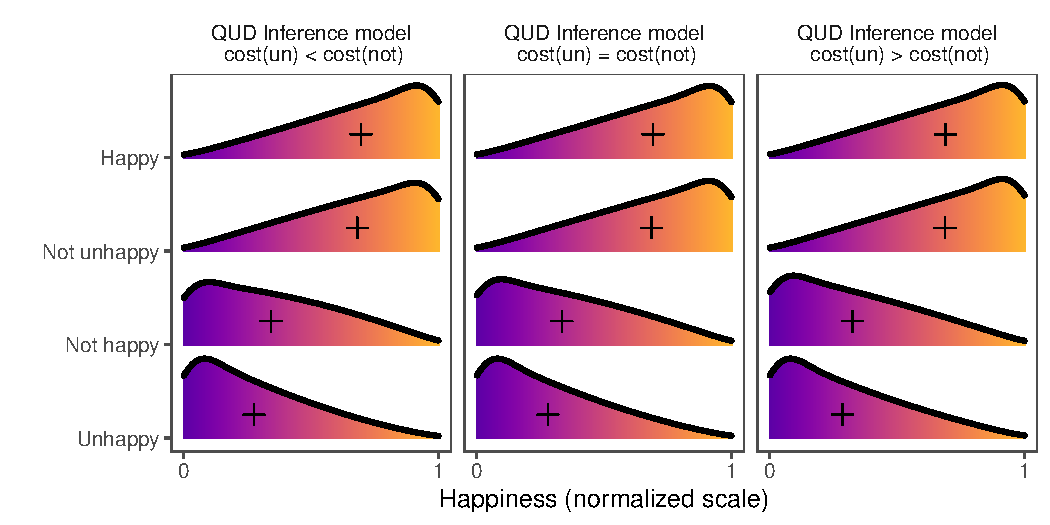
\includegraphics{figs/qud_SI.pdf} 
\caption{QUD based models for the single utterance regime.}.\label{fig:qud}
\end{figure}


\section{Supplementary data analysis}

\subsection{Effect size calculation}


We compute effect sizes by first standardizing the slider responses by subtracting the grand mean $\bar{x}$ and dividing by the standard deviation $SD$:  $\tilde{x} = \frac{x - \bar{x}}{SD}$.
We then model these standardized responses using the same Bayesian regression model that we use for the modeling the raw slider bar data with the one exception that we assume a Gaussian linking function (i.e., standard linear regression) rather than a Beta linking function. 
We then take the samples from the posterior distribution over the relevant contrast and divide those contrasts by the standard deviation (i.e., the $\sigma$ parameter from the Gaussian link in the regression model). 
This procedure returns a distribution over effect sizes, from which we report the mean and 95\% credible interval \cite{kruschke2014doing}. 

%\subsection{Regression results with raw slider ratings}
%
%Here, we report a supplementary analysis which models the raw responses. 
%These regression coefficients are interpretable in terms of the response scale. 
%
%\subsubsection{Experiment 1 results}
%
%Consistent with the results reported in the main text, the difference between the \emph{antonym} vs.~\emph{negated positive} 
%levels of adjective type interacted significantly with antonym type (morphological vs. lexical; \(\beta = \rlgetnum{expt1_helmert_summary.csv}{Rowname}{antonym_typelexical:adjective_type1}{Estimate}{3}\), t\((\rlgetnum{expt1_helmert_summary.csv}{Rowname}{antonym_typelexical:adjective_type1}{df}{0}) = \rlgetnum{expt1_helmert_summary.csv}{Rowname}{antonym_typelexical:adjective_type1}{t.value}{2}, p = \rlgetnum{expt1_helmert_summary.csv}{Rowname}{antonym_typelexical:adjective_type1}{Pr...t..}{3}\)) such that the difference between negated positives and antonyms was stronger for lexical antonyms than morphological antonyms.
%At the same time, the negated positive vs. antonyms contrast was not significantly different for the morphological antonyms (e.g., \emph{unhappy} vs. \emph{not happy}; \(\beta = \rlgetnum{expt1_helmert_summary.csv}{Rowname}{adjective_type1}{Estimate}{3}\), t\((\rlgetnum{expt1_helmert_summary.csv}{Rowname}{adjective_type1}{df}{0}) = \rlgetnum{expt1_helmert_summary.csv}{Rowname}{adjective_type1}{t.value}{2}, p = \rlgetnum{expt1_helmert_summary.csv}{Rowname}{adjective_type1}{Pr...t..}{3}\)).
%Running the same model with the antonym type coded with lexical antonyms as the default level reveals that the negated positive vs. antonyms contrast was significantly different for the lexical antonyms (e.g., \emph{short} vs. \emph{not tall}; \(\beta = \rlgetnum{expt1_helmert_summary_lexBase.csv}{Rowname}{adjective_type1}{Estimate}{3}\), t\((\rlgetnum{expt1_helmert_summary_lexBase.csv}{Rowname}{adjective_type1}{df}{0}) = \rlgetnum{expt1_helmert_summary_lexBase.csv}{Rowname}{adjective_type1}{t.value}{2}, p = \rlgetnum{expt1_helmert_summary_lexBase.csv}{Rowname}{adjective_type1}{Pr...t..}{3}\)).
%
%We observe further that negated morphological antonyms (e.g., \emph{not unhappy}) were rated differently and lower than positives (e.g., \emph{happy}; \(\beta = \rlgetnum{expt1_helmert_summary.csv}{Rowname}{adjective_type3}{Estimate}{3}\), t\((\rlgetnum{expt1_helmert_summary.csv}{Rowname}{adjective_type3}{df}{0}) = \rlgetnum{expt1_helmert_summary.csv}{Rowname}{adjective_type3}{t.value}{2}, p <0.001\)). 
%We additionally observe that negated morphological antonyms (e.g., \emph{not unhappy}) were rated overall lower than negated lexical antonyms (e.g., \emph{not tall}), which manifested as an interaction in the negated antonym vs. positive contrast with the lexical vs. morphological items (\(\beta = \rlgetnum{expt1_helmert_summary.csv}{Rowname}{antonym_typelexical:adjective_type3}{Estimate}{3}\), t\((\rlgetnum{expt1_helmert_summary.csv}{Rowname}{antonym_typelexical:adjective_type3}{df}{0}) = \rlgetnum{expt1_helmert_summary.csv}{Rowname}{antonym_typelexical:adjective_type3}{t.value}{2}, p = \rlgetnum{expt1_helmert_summary.csv}{Rowname}{antonym_typelexical:adjective_type3}{Pr...t..}{3}\)) .
%Negated antonyms received a distinct bimodal distribution wherein most ratings were slightly positive but a minority distribution of ratings were slightly negative (e.g., \emph{not dishonest} meaning \emph{not honest}).
%
%
%
%\subsubsection{Experiment 2 results}
%
%
%As we did in \text{Experiment$\thinspace$1}, we evaluated our hypothesis that, in the \emph{single utterance condition}, morphological antonyms behave like the \emph{\ourmodel} model (i.e., show a partial ordering) while lexical antonyms show a true ordering (like \emph{bonafide contraries}).
%We considered data only from the \emph{single utterances} conditions and built a linear mixed model predicting the raw ratings in terms of \emph{antonym type} (morphological vs.\text{~}lexical; dummy-coded with morphological as the base case), \emph{adjective type} (forward-difference coded in order: antonym, negated positive, negated antonym, positive) and their interaction; the model also included random intercepts and random slopes of \emph{adjective type} by-participant and by-item.
%Consistent with our hypothesis, the \emph{antonym} vs.\text{~}\emph{negated positive} difference was greater for lexical antonyms than morphological antonyms (i.e., an adjective type by antonym type interaction; \(\beta =  \rlgetnum{expt2_glmer_singleUtt.csv}{Rowname}{antonym_typelexant:adj_type1}{Estimate}{3}
%\), SE = 
%\rlgetnum{expt2_glmer_singleUtt.csv}{Rowname}{antonym_typelexant:adj_type1}{Std..Error}{3}, t\(( \rlgetnum{expt2_glmer_singleUtt.csv}{Rowname}{antonym_typelexant:adj_type1}{df}{0}) =  \rlgetnum{expt2_glmer_singleUtt.csv}{Rowname}{antonym_typelexant:adj_type1}{t.value}{2}, p =  \rlgetnum{expt2_glmer_singleUtt.csv}{Rowname}{antonym_typelexant:adj_type1}{Pr...t..}{3}\)).
%Further, the \emph{antonym} vs.\text{~}\emph{negated positive} difference for morphological antonyms (e.g., \emph{unhappy} vs. \emph{not happy}) was not significantly different from zero (\(\beta =  \rlgetnum{expt2_glmer_singleUtt.csv}{Rowname}{adj_type1}{Estimate}{3}
%\), SE = 
%\rlgetnum{expt2_glmer_singleUtt.csv}{Rowname}{adj_type1}{Std..Error}{3}, t\(( \rlgetnum{expt2_glmer_singleUtt.csv}{Rowname}{adj_type1}{df}{0}) =  \rlgetnum{expt2_glmer_singleUtt.csv}{Rowname}{adj_type1}{t.value}{2}, p =  \rlgetnum{expt2_glmer_singleUtt.csv}{Rowname}{adj_type1}{Pr...t..}{3}\)).
%Running the same model with the antonym type coded with lexical antonyms as the default level reveals that the \emph{antonym}~vs.~\emph{negated positive} contrast was significantly different for the lexical antonyms (e.g., \emph{sad} vs. \emph{not happy}; \(\beta =  \rlgetnum{expt2_glmer_singleUtt_lexBase.csv}{Rowname}{adj_type1}{Estimate}{3}
%\), SE = 
%\rlgetnum{expt2_glmer_singleUtt_lexBase.csv}{Rowname}{adj_type1}{Std..Error}{3}, t\(( \rlgetnum{expt2_glmer_singleUtt_lexBase.csv}{Rowname}{adj_type1}{df}{0}) =  \rlgetnum{expt2_glmer_singleUtt_lexBase.csv}{Rowname}{adj_type1}{t.value}{2}, p =  \rlgetnum{expt2_glmer_singleUtt_lexBase.csv}{Rowname}{adj_type1}{Pr...t..}{3}\)).
%
%
%Our second main hypothesis was that context (single vs.\text{~}multiple utterances) modulates the interpretive difference between morphological antonyms and negated positives.
%Specifically, we predict that morphological antonyms will be interpreted more negatively than negated positives in a context with multiple adjectival utterances.
%To evaluate this hypothesis, we considered data only from the morphological antonyms conditions and built a linear mixed model predicting the raw ratings in terms of \emph{adjective type} (forward-difference coded, as above),
%\emph{context} (single vs.~multiple utterances; multiple as base case) and their interaction; the model also included random intercepts and random slopes of adjective type by-participant and by-item.
%The \emph{antonym}~vs.~\emph{negated positive} difference was significantly greater in the \emph{multiple utterances} condition than the \emph{single utterance} condition (i.e., an adjective type by context interaction; \(\beta = \rlgetnum{expt2_glmer_morphological.csv}{Rowname}{conditionimplicit:adj_type1}{Estimate}{3}\), SE = 
%\rlgetnum{expt2_glmer_morphological.csv}{Rowname}{conditionimplicit:adj_type1}{Std..Error}{3}, t\((\rlgetnum{expt2_glmer_morphological.csv}{Rowname}{conditionimplicit:adj_type1}{df}{0}) = \rlgetnum{expt2_glmer_morphological.csv}{Rowname}{conditionimplicit:adj_type1}{t.value}{2}, p < 0.001\)), such that antonyms were interpreted more negatively than negated positives in the multiple utterances condition (\(\beta = \rlgetnum{expt2_glmer_morphological.csv}{Rowname}{adj_type1}{Estimate}{3}\), SE = 
%\rlgetnum{expt2_glmer_morphological.csv}{Rowname}{adj_type1}{Std..Error}{3}, t\((\rlgetnum{expt2_glmer_morphological.csv}{Rowname}{adj_type1}{df}{0}) = \rlgetnum{expt2_glmer_morphological.csv}{Rowname}{adj_type1}{t.value}{2}, p < 0.001\)), but not in the single utterance condition (same contrast as previous paragraph).
%
%The predictions of the \ourmodel model are ambiguous about the relevant three-way interaction (\emph{antonym} vs.~\emph{negated positive} by lexical vs.~morphological adjective type by context).
%On the one hand, for the \emph{antonym} vs.~\emph{negated positive} contrast, the model predicts no difference in meaning for morphological antonyms when presented in isolation, but does predict meaning differences when the alternatives are presented together, whereas the difference is expected to occur for lexical antonyms in both context conditions.
%On the other hand, the model's inferences about the likely meaning of all of the adjectives gets further differentiated as a result of being presented in the same context (i.e., all adjectives get more specific interpretations).
%Thus, it is not clear \emph{a priori} that the \ourmodel model predicts a three-way interaction nor the direction of the interaction.
%As an exploratory analysis, we examined these effects in a full three-way interactive model and found the relevant three-way interaction was in the direction of lexical antonyms showing a larger \emph{antonym} vs.~\emph{negated positive} difference in the multiple utterance condition; this effect was not significant, though (\(\beta =  \rlgetnum{expt2_glmer_full3way.csv}{Rowname}{adj_type1:antonym_typelexant:conditionexplicit}{Estimate}{3}
%\), SE = 
%\rlgetnum{expt2_glmer_full3way.csv}{Rowname}{adj_type1:antonym_typelexant:conditionexplicit}{Std..Error}{3}, t\(( \rlgetnum{expt2_glmer_full3way.csv}{Rowname}{adj_type1:antonym_typelexant:conditionexplicit}{df}{0}) =  \rlgetnum{expt2_glmer_full3way.csv}{Rowname}{adj_type1:antonym_typelexant:conditionexplicit}{t.value}{2}, p =  \rlgetnum{expt2_glmer_full3way.csv}{Rowname}{adj_type1:antonym_typelexant:conditionexplicit}{Pr...t..}{3}\)).
%%\mf{maybe this paragraph could, if absolutely necessary, be dropped to save space?}
%
%
%
%
%\subsubsection{Experiment 3 results}


\subsection{Item analysis}

Below, we show the item variability in the data sets.

%\subsection{Experiment 1}

%\subsubsection{Morphological antonym pairs}


\begin{figure}[t]
\centering 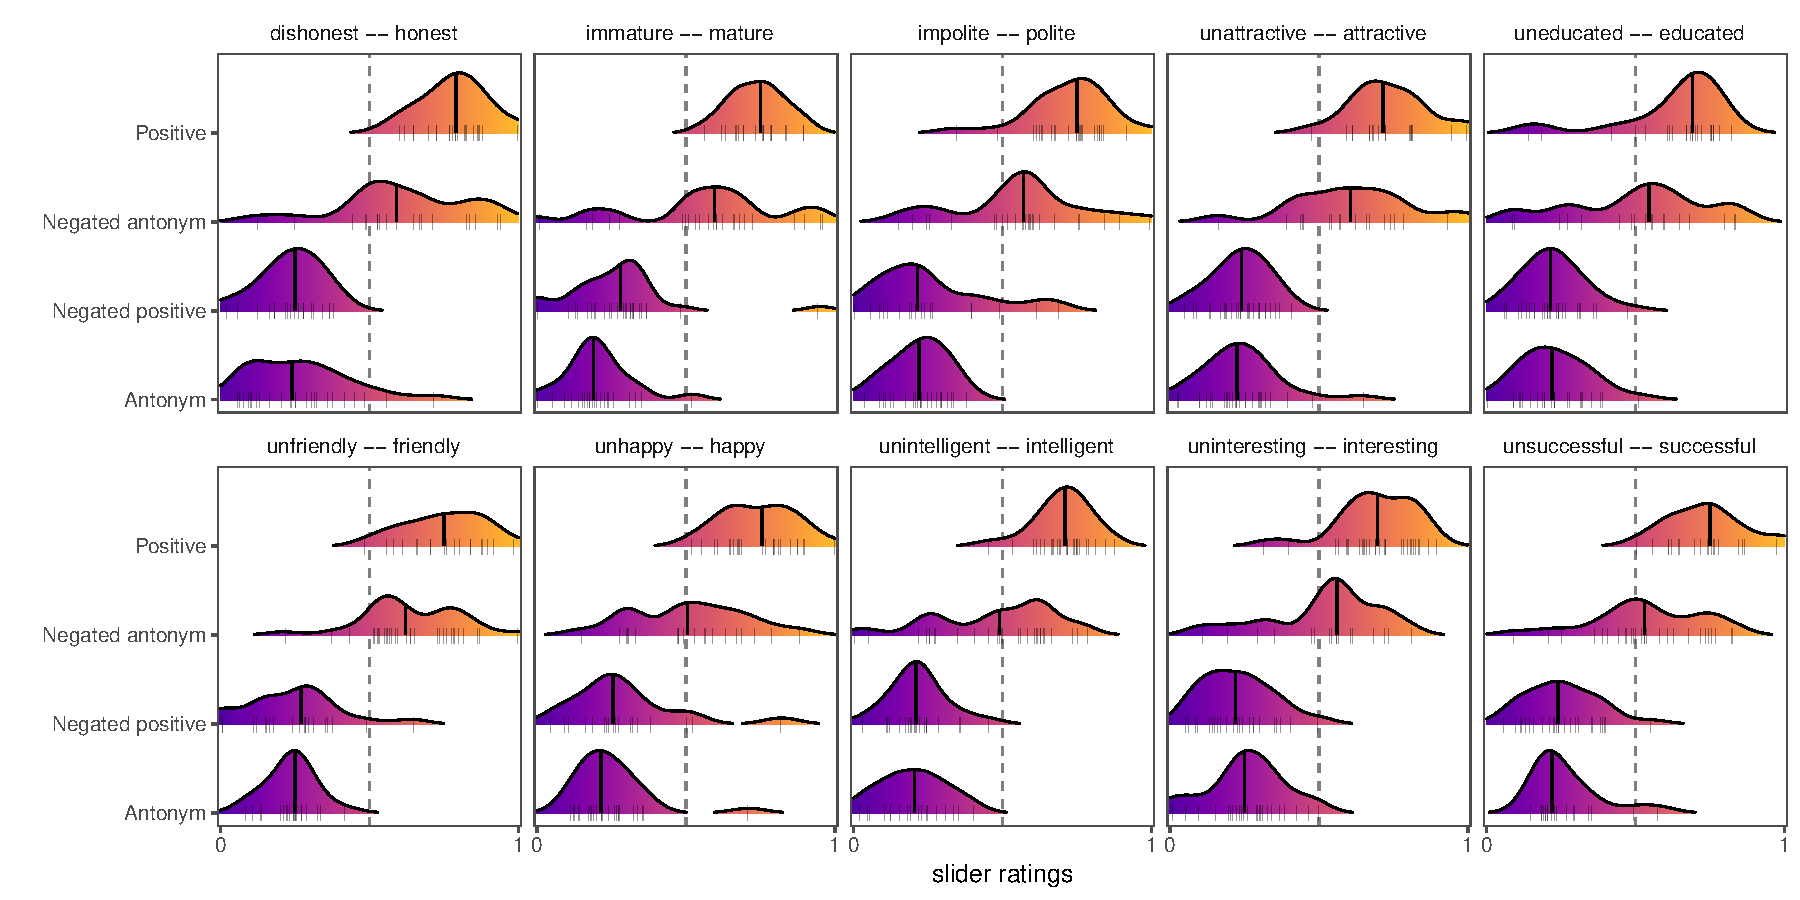
\includegraphics{figs/cogsci_expt1_morph_byItem_densities.pdf} 
\caption{Results by item for Experiment 1, morphological antonym pairs.}.\label{fig:items_morph_expt1}
\end{figure}


%\subsubsection{Lexical antonym pairs}

\begin{figure}[t]
\centering 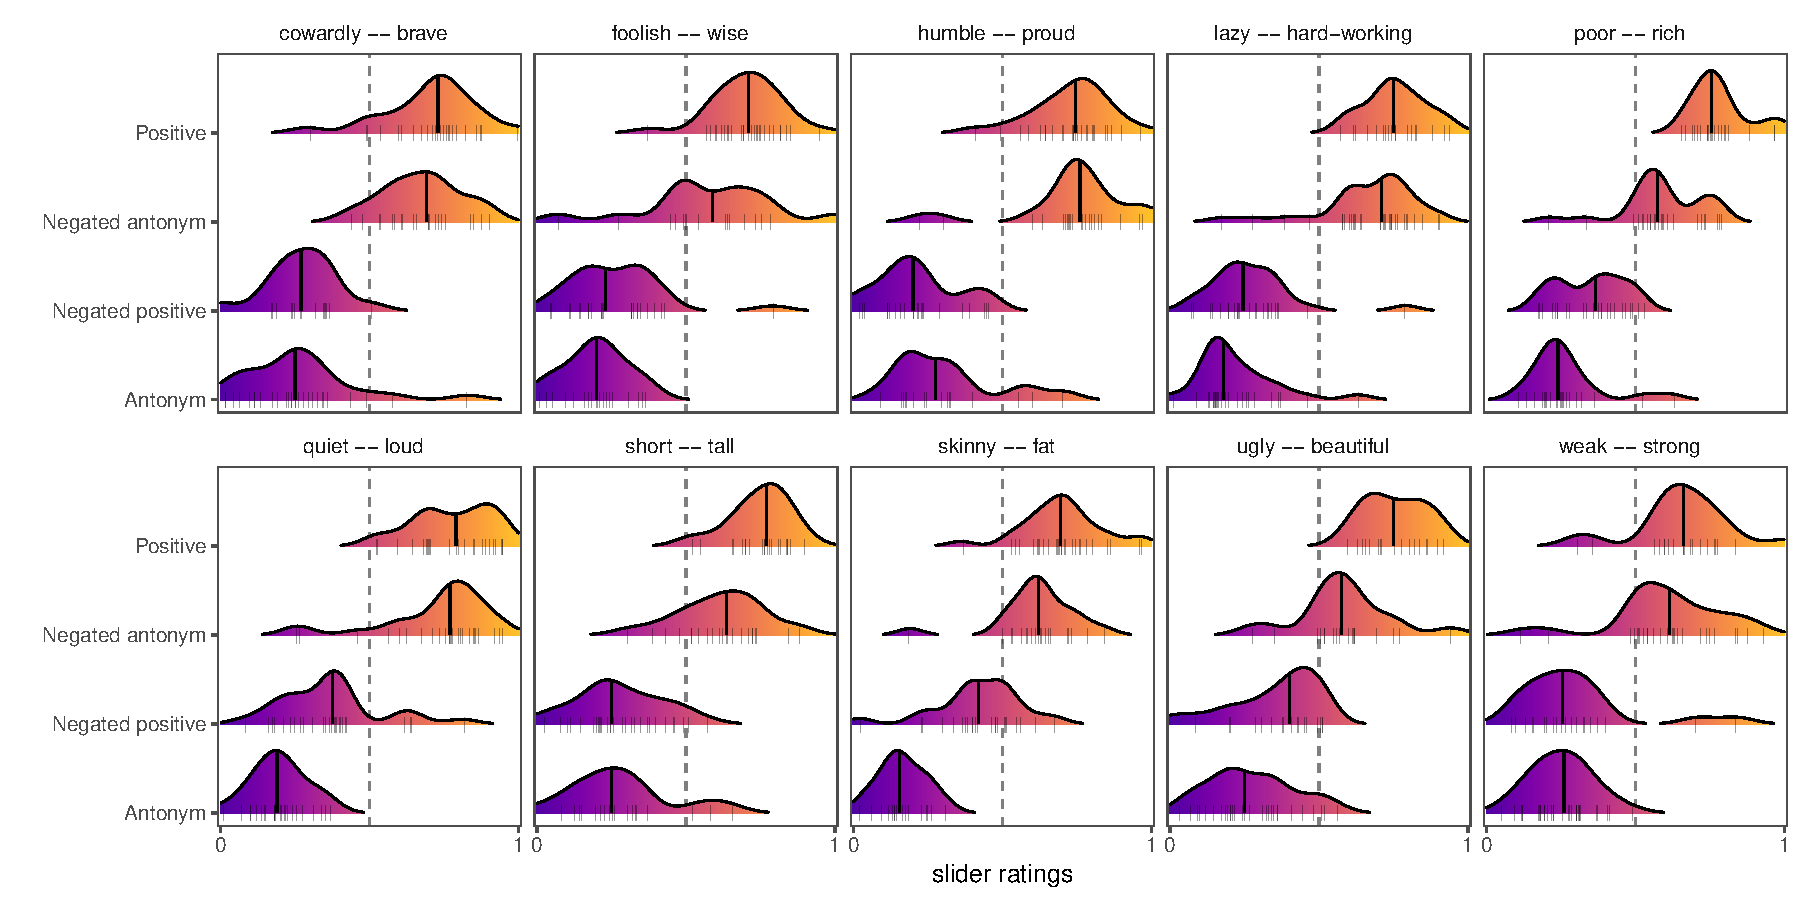
\includegraphics{figs/cogsci_expt1_lex_byItem_densities.pdf} 
\caption{Results by item for Experiment 1, lexical antonym pairs.}.\label{fig:items_lex_expt1}

\end{figure}




%\subsection{Experiment 2}

%\subsubsection{Single utterance condition: Morphological antonym pairs}


We draw particular attention to Figure \ref{fig:items_morph_singleUtt_expt2}, which shows the by-item results for the morphological antonym pairs from the single utterance condition (each rating presented to the participant in isolation). Ratings for \emph{positive} adjectives (e.g., happy, forgiving) are highly consistent across items, though some items (e.g., affectionate) have a hint of bi-modality, which might indicate pragmatic competition with a stronger scalar alternative \cite<e.g., loving; >{van2016scalar}. Negated positives (e.g., \emph{not happy}) are also largely consistent, again with some items (e.g., attractive) indicating a bi-modal distribution of responses, with one of the modes consistent with an effect of \emph{negative strengthening} \cite<cf.,>{Ruytenbeek2017, Gotzner2018}. Such bi-modalities also appears for the morphological antonym for some items (e.g., \emph{intolerant}). These bimodalities for negated positives and morphological antonyms are convergent evidence for our \ourmodel account, wherein listeners entertain multiple possible meanings for negation markers. 

%\subsubsection{Single utterance condition: Lexical antonym pairs}

%\subsubsection{Multiple utterance condition: Morphological antonym pairs}

%\subsubsection{Multiple utterance condition: Lexical antonym pairs}

%\subsection{Experiment 3}


\begin{figure}[t]
\centering 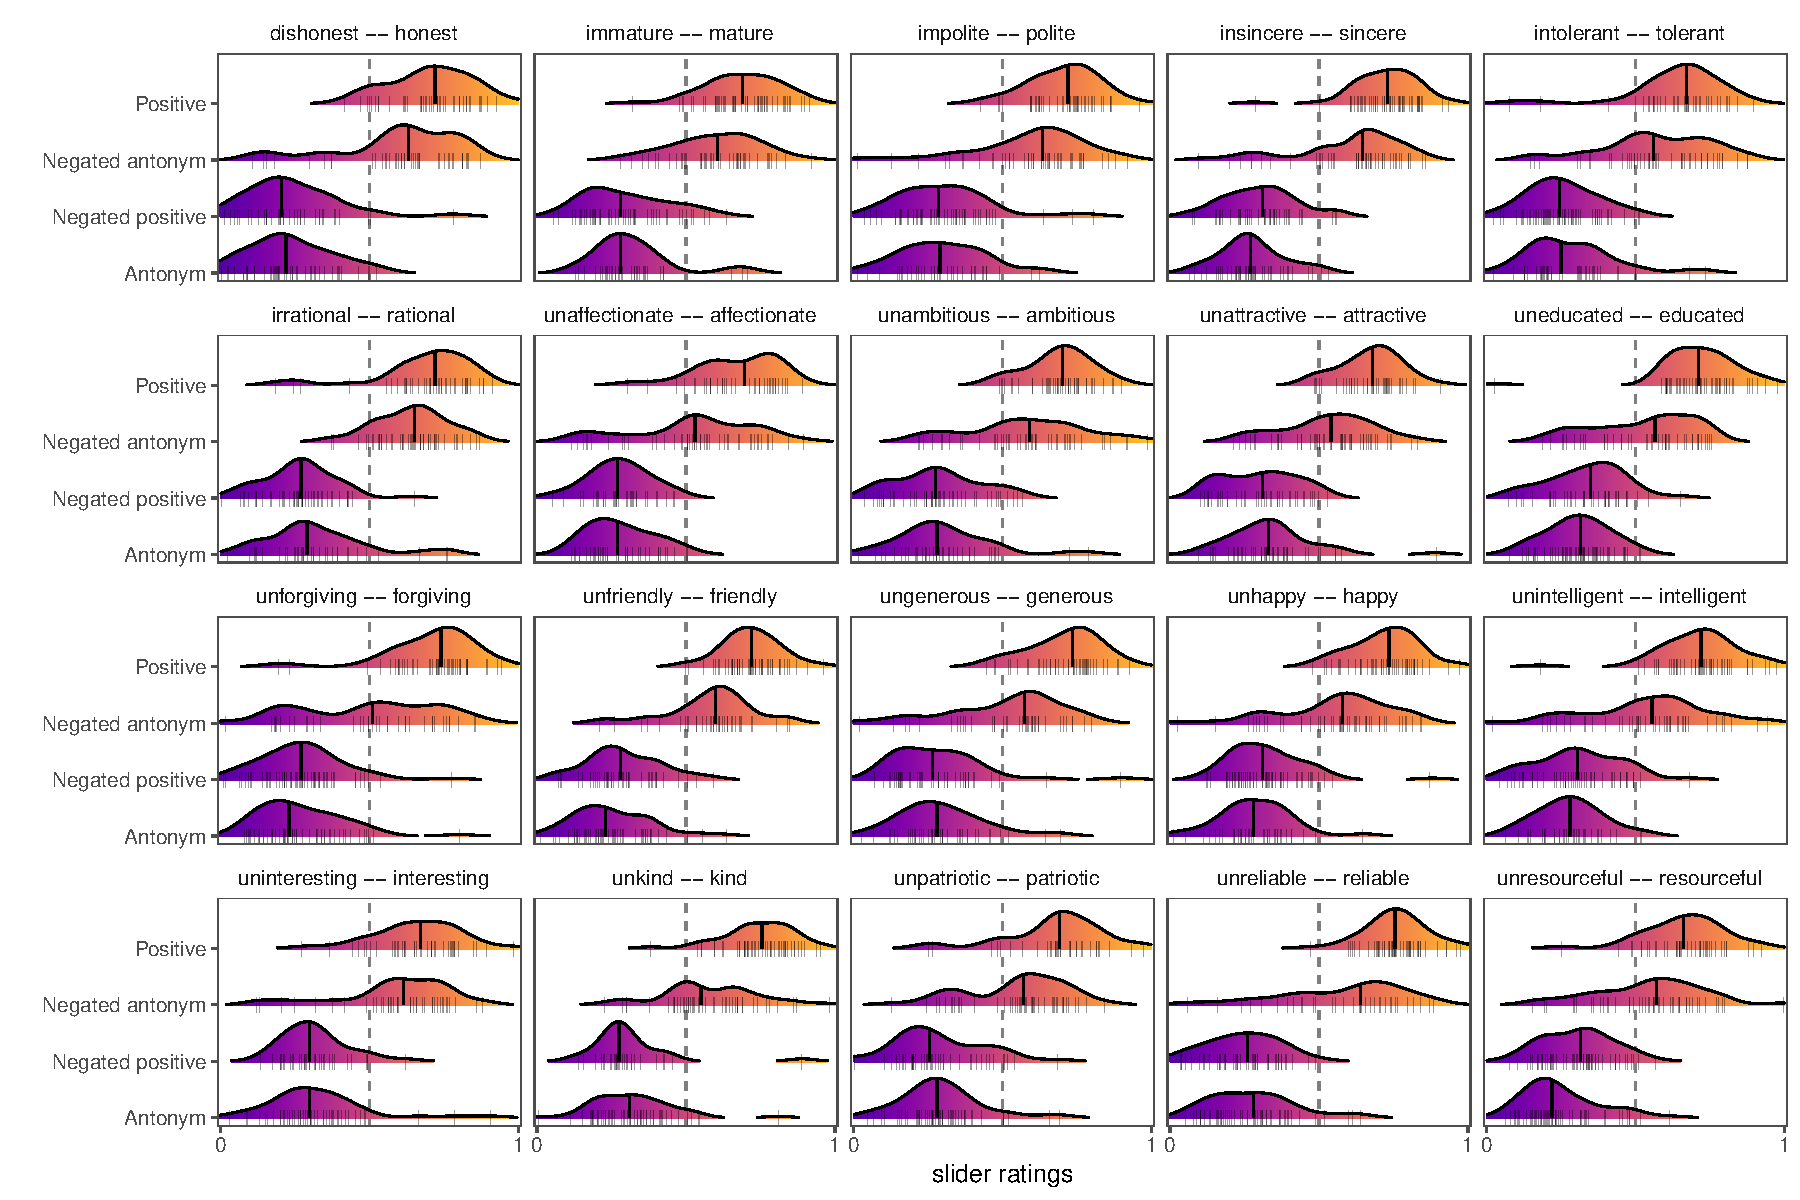
\includegraphics{figs/cogsci_expt2_morph_singleUtt_byItem_densities.pdf} 
\caption{Results by item for Experiment 2, morphological antonym pairs, single utterance condition.}.\label{fig:items_morph_singleUtt_expt2}
\end{figure}

\begin{figure}[t]
\centering 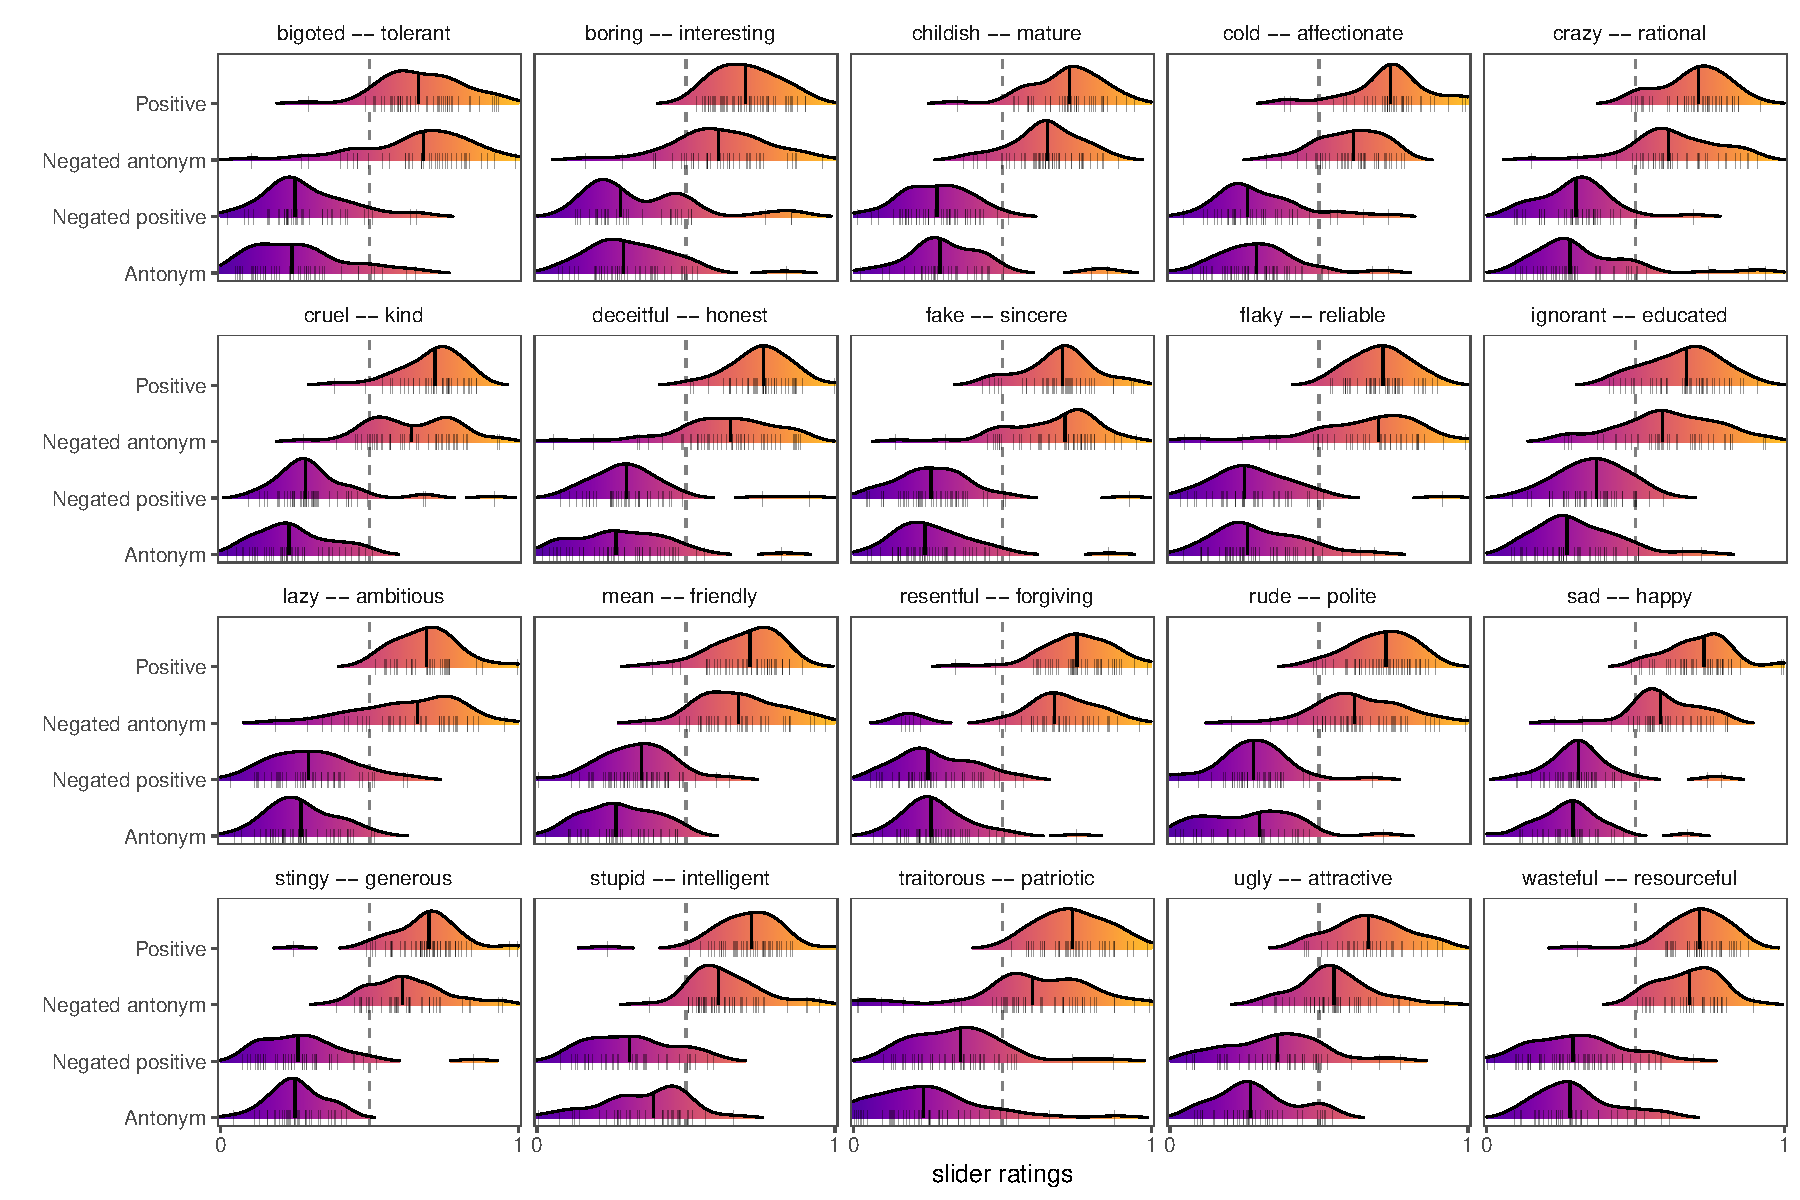
\includegraphics{figs/cogsci_expt2_lex_singleUtt_byItem_densities.pdf} 
\caption{Results by item for Experiment 2, lexical antonym pairs, single utterance condition.}.\label{fig:items_lex_singleUtt_expt2}
\end{figure}

\begin{figure}[t]
\centering 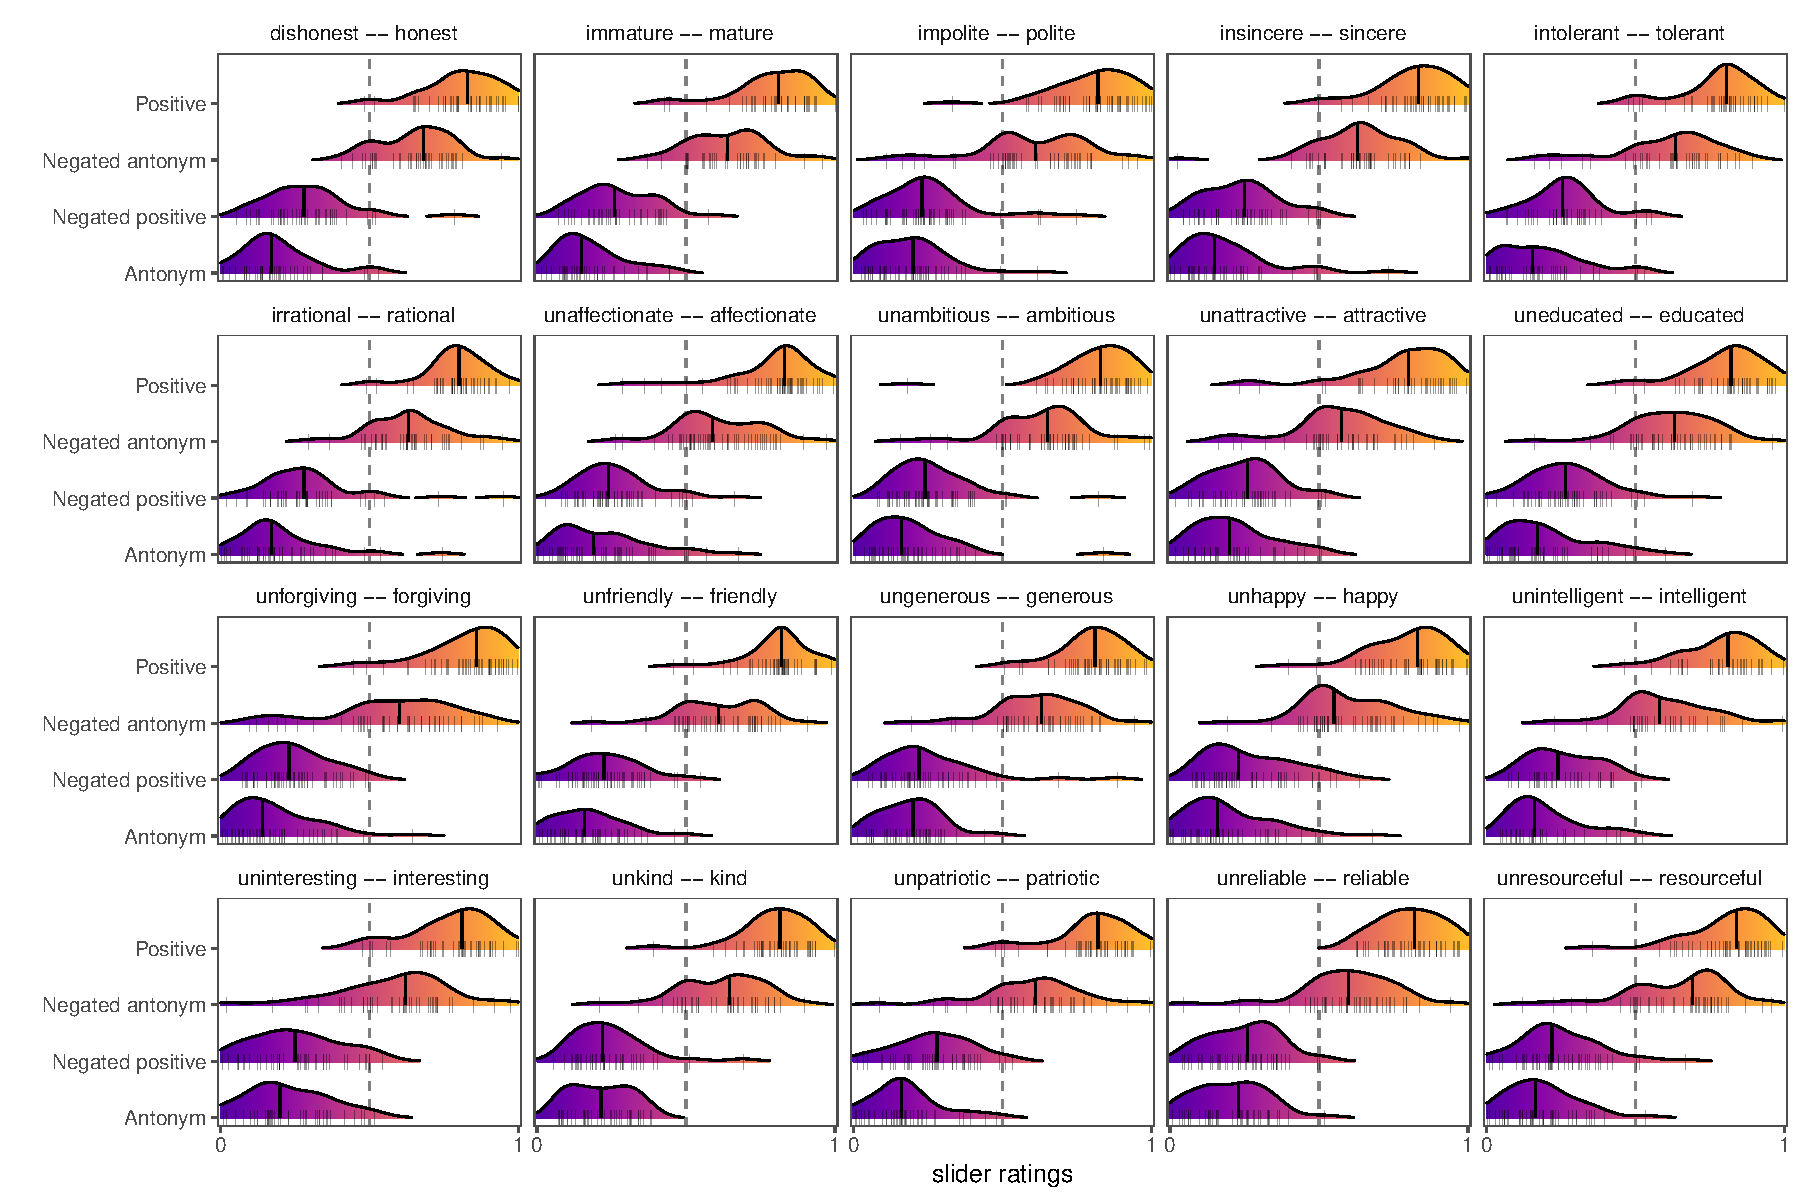
\includegraphics{figs/cogsci_expt2_morph_multiUtt_byItem_densities.pdf} 
\caption{Results by item for Experiment 2, morphological antonym pairs, multiple utterance condition.}.\label{fig:items_morph_multiUtt_expt2}
\end{figure}

\begin{figure}[t]
\centering 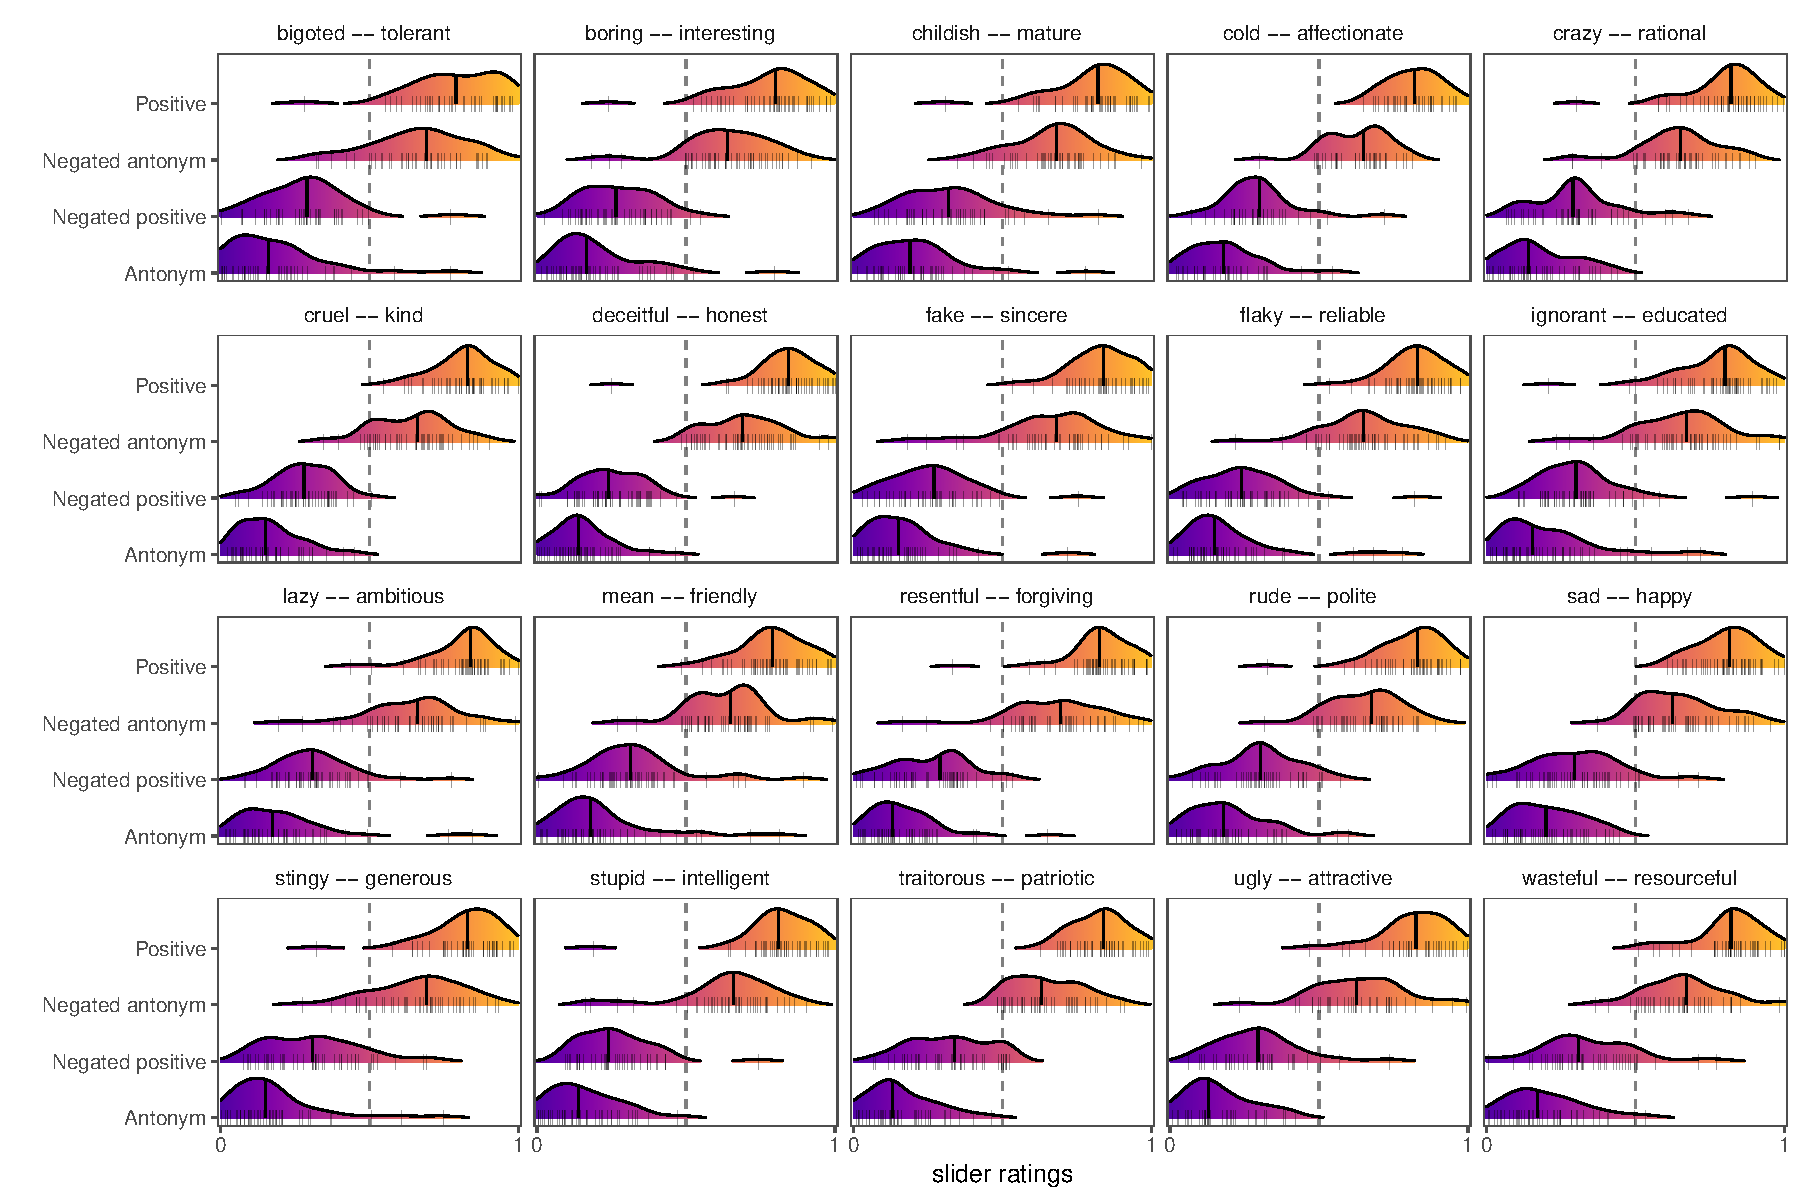
\includegraphics{figs/cogsci_expt2_lex_multiUtt_byItem_densities.pdf} 
\caption{Results by item for Experiment 2, lexical antonym pairs, multiple utterance condition.}.\label{fig:items_lex_multiUtt_expt2}
\end{figure}


%\subsection{Experiment 3}


\begin{figure}[t]
\centering 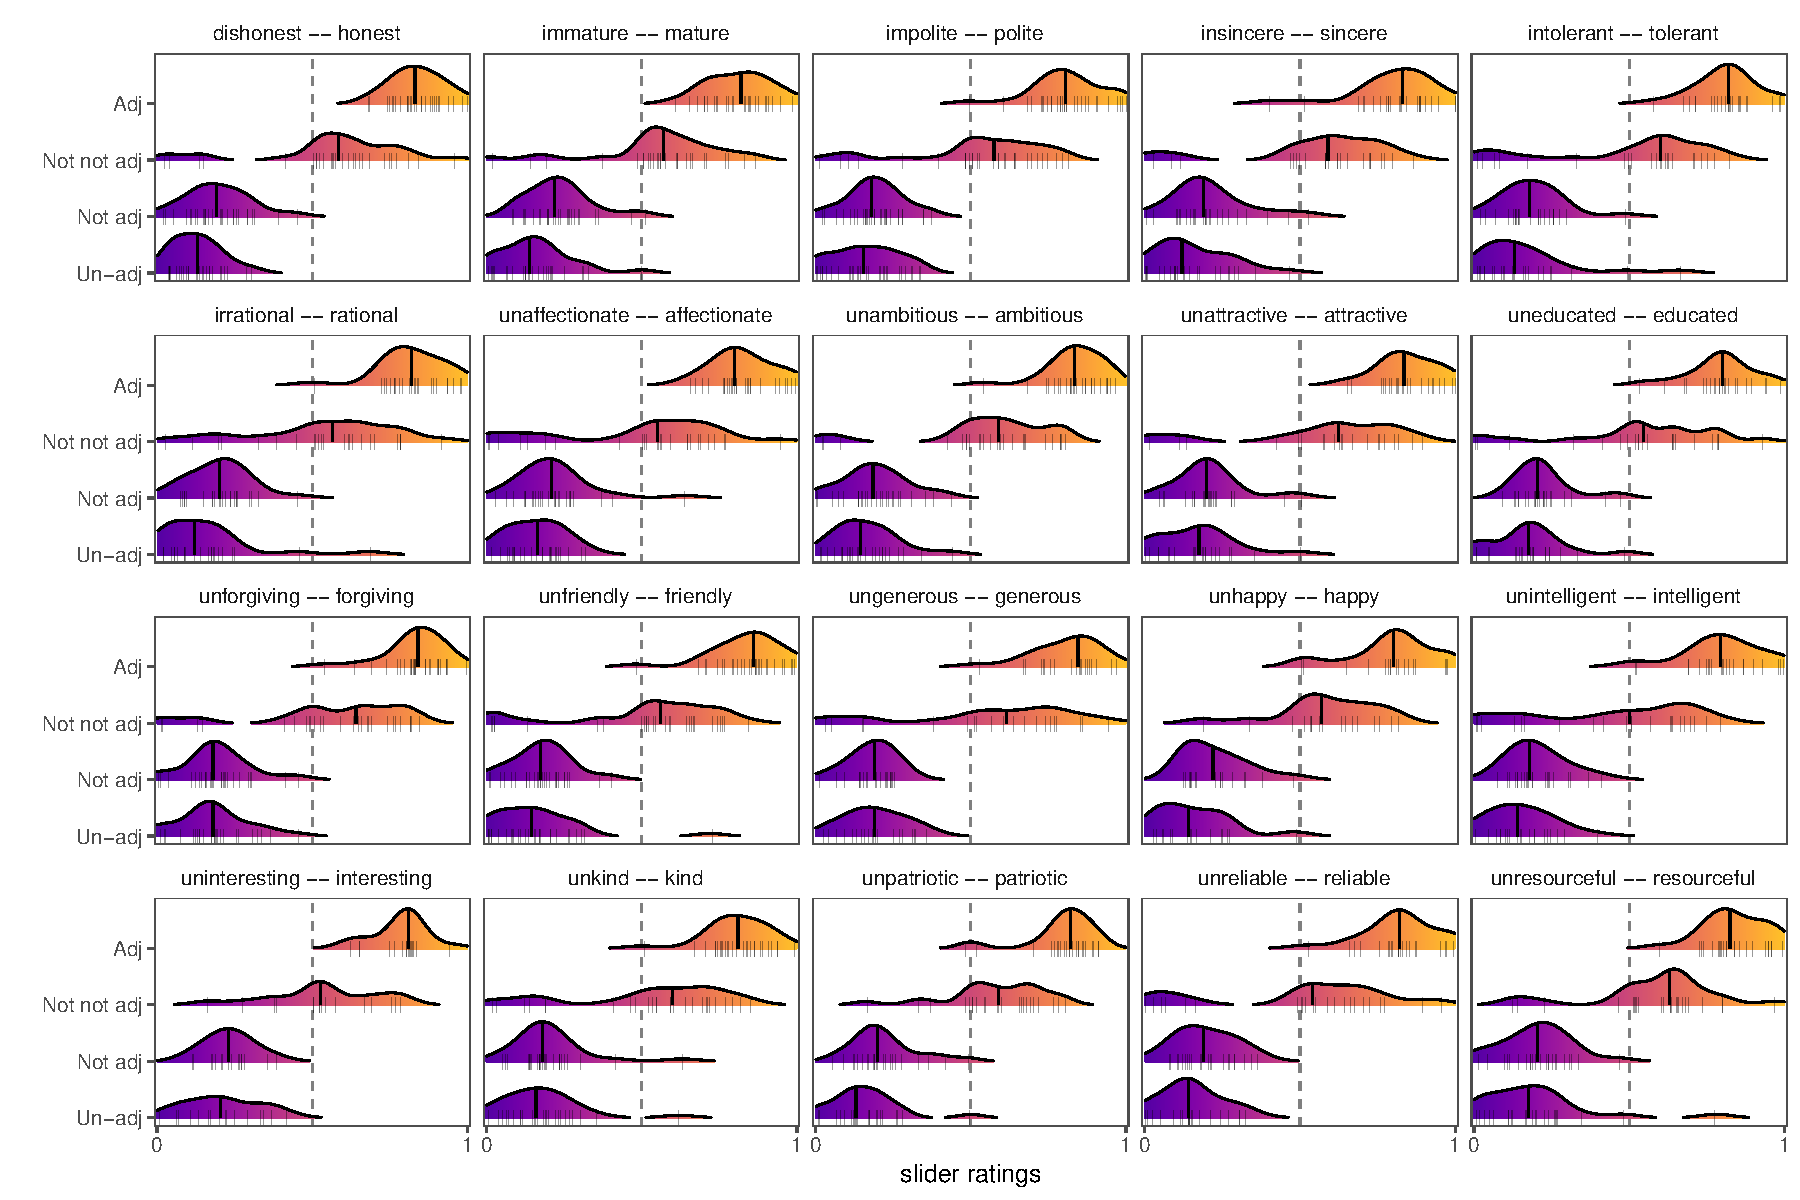
\includegraphics{figs/expt3_byItem_densities.pdf}
\caption{Results by item for Experiment 3a.}.\label{fig:items_expt3}
\end{figure}



\newpage

%\hypertarget{references}{%
%\section{References}\label{references}%}

\bibliographystyle{apacite}

\setlength{\bibleftmargin}{.125in}
\setlength{\bibindent}{-\bibleftmargin}

\bibliography{negant}

%\begingroup
%\setlength{\parindent}{-0.5in}
%\setlength{\leftskip}{0.5in}
%
%\hypertarget{refs}{}
%\leavevmode\hypertarget{ref-lme4}{}%
%Bates, D., M\wrapmf{\"{a}}chler, M., Bolker, B., \& Walker, S. (2015). Fitting linear mixed-effects models using lme4. \emph{Journal of Statistical Software}, \emph{67}(1), 1--48.
%
%\leavevmode\hypertarget{ref-Bergen2016}{}%
%Bergen, L., Levy, R., \& Goodman, N. D. (2016). Pragmatic reasoning through semantic inference. \emph{Semantics and Pragmatics}, \emph{9}.
%
%\leavevmode\hypertarget{ref-Blutner2004:pragmatics}{}%
%Blutner, R. (2004). Pragmatics and the lexicon. \emph{Handbook of Pragmatics}, \emph{488514}.
%
%\leavevmode\hypertarget{ref-bybee2006usage}{}%
%Bybee, J. L. (2006). From usage to grammar: The mind's response to repetition. \emph{Language}, \emph{82}(4), 711--733.
%
%\leavevmode\hypertarget{ref-Cable2017}{}%
%Cable, S. (2017). The good, the 'not good', and the 'not pretty': Negation in the negative predicates of tlingit.
%
%\leavevmode\hypertarget{ref-Franke2015a}{}%
%Franke, M., \& J\wrapmf{\"{a}}ger, G. (2015). Probabilistic pragmatics, or why Bayes' rule is probably important for pragmatics. In \emph{Zeitschrift für sprachwissenschaft} (pp. 3--44).
%
%\leavevmode\hypertarget{ref-Goodman2016:RSA}{}%
%Goodman, N. D., \& Frank, M. C. (2016). Pragmatic language interpretation as probabilistic inference. \emph{Trends in Cognitive Sciences}, \emph{20}(11), 818--829.
%
%\leavevmode\hypertarget{ref-Horn1989:Natural}{}%
%Horn, L. R. (1989). \emph{A natural history of negation}. University of Chicago Press.
%
%\leavevmode\hypertarget{ref-Horn1991:Duplex}{}%
%Horn, L. R. (1991). Duplex negatio affirmat...: the economy of double negation. \emph{CLS 27-II: Papers from the Parasession on Negation}, 80--106.
%
%\leavevmode\hypertarget{ref-Jespersen1917:Negation}{}%
%Jespersen, O. (1917). \emph{Negation in english and other languages}. Kobenhavn: Host.
%
%\leavevmode\hypertarget{ref-Jespersen1924}{}%
%Jespersen, O. (1924). \emph{The philosophy of grammar}. London: Allen \& Unwin.
%
%\leavevmode\hypertarget{ref-Kennedy2007}{}%
%Kennedy, C. (2007). Vagueness and grammar: the semantics of relative and absolute gradable adjectives. \emph{Linguistics and Philosophy}, \emph{30}, 1--35.
%
%\leavevmode\hypertarget{ref-Krifka2007:Negated-antonyms}{}%
%Krifka, M. (2007). Negated Antonyms: Creating and Filling the Gap. \emph{Presupposition and Implicature in Compositional Semantics}, 163--177.
%
%\leavevmode\hypertarget{ref-Lassiter2015}{}%
%Lassiter, D., \& Goodman, N. D. (2015). Adjectival vagueness in a Bayesian model of interpretation. \emph{Synthese}.
%
%\leavevmode\hypertarget{ref-Markman1989}{}%
%Markman, E. M. (1989). \emph{Categorization and naming in children: Problems of induction}. MIT Press.
%
%\leavevmode\hypertarget{ref-MorganLevy2016:binomials}{}%
%Morgan, E., \& Levy, R. (2016). Abstract knowledge versus direct experience in processing of binomial expressions. \emph{Cognition}, \emph{157}, 384--402.
%
%\leavevmode\hypertarget{ref-Odonnell2015productivity}{}%
%O'Donnell, T. J. (2015). \emph{Productivity and reuse in language: A theory of linguistic computation and storage}. MIT Press.
%
%\leavevmode\hypertarget{ref-Rett2014:eval}{}%
%Rett, J. (2014). \emph{The semantics of evaluativity}. Oxford University Press.
%
%\leavevmode\hypertarget{ref-Yoon2017}{}%
%Yoon, E. J., Tessler, M. H., Goodman, N. D., \& Frank, M. C. (2017). "I won't lie, it wasn't amazing": Modeling polite indirect speech. In \emph{Proceedings of the 39th annual meeting of the cognitive science society}.
%
%\endgroup


\end{document}
